\documentclass[twoside]{book}

% Packages required by doxygen
\usepackage{fixltx2e}
\usepackage{calc}
\usepackage{doxygen}
\usepackage[export]{adjustbox} % also loads graphicx
\usepackage{graphicx}
\usepackage[utf8]{inputenc}
\usepackage{makeidx}
\usepackage{multicol}
\usepackage{multirow}
\PassOptionsToPackage{warn}{textcomp}
\usepackage{textcomp}
\usepackage[nointegrals]{wasysym}
\usepackage[table]{xcolor}

% Font selection
\usepackage[T1]{fontenc}
\usepackage[scaled=.90]{helvet}
\usepackage{courier}
\usepackage{amssymb}
\usepackage{sectsty}
\renewcommand{\familydefault}{\sfdefault}
\allsectionsfont{%
  \fontseries{bc}\selectfont%
  \color{darkgray}%
}
\renewcommand{\DoxyLabelFont}{%
  \fontseries{bc}\selectfont%
  \color{darkgray}%
}
\newcommand{\+}{\discretionary{\mbox{\scriptsize$\hookleftarrow$}}{}{}}

% Page & text layout
\usepackage{geometry}
\geometry{%
  a4paper,%
  top=2.5cm,%
  bottom=2.5cm,%
  left=2.5cm,%
  right=2.5cm%
}
\tolerance=750
\hfuzz=15pt
\hbadness=750
\setlength{\emergencystretch}{15pt}
\setlength{\parindent}{0cm}
\setlength{\parskip}{3ex plus 2ex minus 2ex}
\makeatletter
\renewcommand{\paragraph}{%
  \@startsection{paragraph}{4}{0ex}{-1.0ex}{1.0ex}{%
    \normalfont\normalsize\bfseries\SS@parafont%
  }%
}
\renewcommand{\subparagraph}{%
  \@startsection{subparagraph}{5}{0ex}{-1.0ex}{1.0ex}{%
    \normalfont\normalsize\bfseries\SS@subparafont%
  }%
}
\makeatother

% Headers & footers
\usepackage{fancyhdr}
\pagestyle{fancyplain}
\fancyhead[LE]{\fancyplain{}{\bfseries\thepage}}
\fancyhead[CE]{\fancyplain{}{}}
\fancyhead[RE]{\fancyplain{}{\bfseries\leftmark}}
\fancyhead[LO]{\fancyplain{}{\bfseries\rightmark}}
\fancyhead[CO]{\fancyplain{}{}}
\fancyhead[RO]{\fancyplain{}{\bfseries\thepage}}
\fancyfoot[LE]{\fancyplain{}{}}
\fancyfoot[CE]{\fancyplain{}{}}
\fancyfoot[RE]{\fancyplain{}{\bfseries\scriptsize Generated by Doxygen }}
\fancyfoot[LO]{\fancyplain{}{\bfseries\scriptsize Generated by Doxygen }}
\fancyfoot[CO]{\fancyplain{}{}}
\fancyfoot[RO]{\fancyplain{}{}}
\renewcommand{\footrulewidth}{0.4pt}
\renewcommand{\chaptermark}[1]{%
  \markboth{#1}{}%
}
\renewcommand{\sectionmark}[1]{%
  \markright{\thesection\ #1}%
}

% Indices & bibliography
\usepackage{natbib}
\usepackage[titles]{tocloft}
\setcounter{tocdepth}{3}
\setcounter{secnumdepth}{5}
\makeindex

% Hyperlinks (required, but should be loaded last)
\usepackage{ifpdf}
\ifpdf
  \usepackage[pdftex,pagebackref=true]{hyperref}
\else
  \usepackage[ps2pdf,pagebackref=true]{hyperref}
\fi
\hypersetup{%
  colorlinks=true,%
  linkcolor=blue,%
  citecolor=blue,%
  unicode%
}

% Custom commands
\newcommand{\clearemptydoublepage}{%
  \newpage{\pagestyle{empty}\cleardoublepage}%
}

\usepackage{caption}
\captionsetup{labelsep=space,justification=centering,font={bf},singlelinecheck=off,skip=4pt,position=top}

%===== C O N T E N T S =====

\begin{document}

% Titlepage & ToC
\hypersetup{pageanchor=false,
             bookmarksnumbered=true,
             pdfencoding=unicode
            }
\pagenumbering{alph}
\begin{titlepage}
\vspace*{7cm}
\begin{center}%
{\Large Backup Enterprise Pro }\\
\vspace*{1cm}
{\large Generated by Doxygen 1.8.13}\\
\end{center}
\end{titlepage}
\clearemptydoublepage
\pagenumbering{roman}
\tableofcontents
\clearemptydoublepage
\pagenumbering{arabic}
\hypersetup{pageanchor=true}

%--- Begin generated contents ---
\chapter{Hierarchical Index}
\section{Class Hierarchy}
This inheritance list is sorted roughly, but not completely, alphabetically\+:\begin{DoxyCompactList}
\item \contentsline{section}{A\+PI}{\pageref{class_a_p_i}}{}
\begin{DoxyCompactList}
\item \contentsline{section}{Backup\+A\+PI}{\pageref{class_backup_a_p_i}}{}
\end{DoxyCompactList}
\item \contentsline{section}{Auth}{\pageref{class_auth}}{}
\item \contentsline{section}{Backup\+A\+P\+I\+Session}{\pageref{class_backup_a_p_i_session}}{}
\item \contentsline{section}{Backup\+Database}{\pageref{class_backup_database}}{}
\item \contentsline{section}{Backup\+:\+:File\+:\+:Backup\+File}{\pageref{class_backup_1_1_file_1_1_backup_file}}{}
\item \contentsline{section}{Backup\+File}{\pageref{class_backup_file}}{}
\item \contentsline{section}{Backup\+L\+D\+AP}{\pageref{class_backup_l_d_a_p}}{}
\item \contentsline{section}{Backup\+Log}{\pageref{class_backup_log}}{}
\item \contentsline{section}{Backup\+Machine}{\pageref{class_backup_machine}}{}
\item \contentsline{section}{Backup\+Session}{\pageref{class_backup_session}}{}
\item \contentsline{section}{Backup\+Upload}{\pageref{class_backup_upload}}{}
\item \contentsline{section}{Backup\+User}{\pageref{class_backup_user}}{}
\item \contentsline{section}{Backup\+:\+:Networking\+:\+:Client}{\pageref{class_backup_1_1_networking_1_1_client}}{}
\item \contentsline{section}{Backup\+:\+:Compression\+:\+:Compressor}{\pageref{class_backup_1_1_compression_1_1_compressor}}{}
\item enable\+\_\+shared\+\_\+from\+\_\+this\begin{DoxyCompactList}
\item \contentsline{section}{Backup\+:\+:Networking\+:\+:Connection}{\pageref{class_backup_1_1_networking_1_1_connection}}{}
\end{DoxyCompactList}
\item \contentsline{section}{Backup\+:\+:Types\+:\+:file\+\_\+data}{\pageref{struct_backup_1_1_types_1_1file__data}}{}
\item \contentsline{section}{Backup\+:\+:Types\+:\+:file\+\_\+directory}{\pageref{struct_backup_1_1_types_1_1file__directory}}{}
\item \contentsline{section}{Backup\+:\+:File\+:\+:File\+Iterator}{\pageref{class_backup_1_1_file_1_1_file_iterator}}{}
\item \contentsline{section}{Backup\+:\+:Types\+:\+:http\+\_\+request}{\pageref{struct_backup_1_1_types_1_1http__request}}{}
\item \contentsline{section}{Backup\+:\+:Types\+:\+:http\+\_\+upload\+\_\+file}{\pageref{struct_backup_1_1_types_1_1http__upload__file}}{}
\item \contentsline{section}{Backup\+:\+:Networking\+:\+:Http\+Request}{\pageref{class_backup_1_1_networking_1_1_http_request}}{}
\item \contentsline{section}{Backup\+:\+:Database\+:\+:Local\+Database}{\pageref{class_backup_1_1_database_1_1_local_database}}{}
\item \contentsline{section}{Backup\+:\+:Logging\+:\+:Log}{\pageref{class_backup_1_1_logging_1_1_log}}{}
\item \contentsline{section}{Backup\+:\+:Networking\+:\+:Server}{\pageref{class_backup_1_1_networking_1_1_server}}{}
\item \contentsline{section}{Backup\+:\+:Compression\+:\+:Tarball}{\pageref{class_backup_1_1_compression_1_1_tarball}}{}
\end{DoxyCompactList}

\chapter{Class Index}
\section{Class List}
Here are the classes, structs, unions and interfaces with brief descriptions\+:\begin{DoxyCompactList}
\item\contentsline{section}{\hyperlink{class_a_p_i}{A\+PI} }{\pageref{class_a_p_i}}{}
\item\contentsline{section}{\hyperlink{class_auth}{Auth} }{\pageref{class_auth}}{}
\item\contentsline{section}{\hyperlink{class_backup_a_p_i}{Backup\+A\+PI} }{\pageref{class_backup_a_p_i}}{}
\item\contentsline{section}{\hyperlink{class_backup_a_p_i_session}{Backup\+A\+P\+I\+Session} }{\pageref{class_backup_a_p_i_session}}{}
\item\contentsline{section}{\hyperlink{class_backup_database}{Backup\+Database} }{\pageref{class_backup_database}}{}
\item\contentsline{section}{\hyperlink{class_backup_1_1_file_1_1_backup_file}{Backup\+::\+File\+::\+Backup\+File} }{\pageref{class_backup_1_1_file_1_1_backup_file}}{}
\item\contentsline{section}{\hyperlink{class_backup_file}{Backup\+File} }{\pageref{class_backup_file}}{}
\item\contentsline{section}{\hyperlink{class_backup_l_d_a_p}{Backup\+L\+D\+AP} }{\pageref{class_backup_l_d_a_p}}{}
\item\contentsline{section}{\hyperlink{class_backup_log}{Backup\+Log} }{\pageref{class_backup_log}}{}
\item\contentsline{section}{\hyperlink{class_backup_machine}{Backup\+Machine} }{\pageref{class_backup_machine}}{}
\item\contentsline{section}{\hyperlink{class_backup_session}{Backup\+Session} }{\pageref{class_backup_session}}{}
\item\contentsline{section}{\hyperlink{class_backup_upload}{Backup\+Upload} }{\pageref{class_backup_upload}}{}
\item\contentsline{section}{\hyperlink{class_backup_user}{Backup\+User} }{\pageref{class_backup_user}}{}
\item\contentsline{section}{\hyperlink{class_backup_1_1_networking_1_1_client}{Backup\+::\+Networking\+::\+Client} }{\pageref{class_backup_1_1_networking_1_1_client}}{}
\item\contentsline{section}{\hyperlink{class_backup_1_1_compression_1_1_compressor}{Backup\+::\+Compression\+::\+Compressor} }{\pageref{class_backup_1_1_compression_1_1_compressor}}{}
\item\contentsline{section}{\hyperlink{class_backup_1_1_networking_1_1_connection}{Backup\+::\+Networking\+::\+Connection} }{\pageref{class_backup_1_1_networking_1_1_connection}}{}
\item\contentsline{section}{\hyperlink{struct_backup_1_1_types_1_1file__data}{Backup\+::\+Types\+::file\+\_\+data} }{\pageref{struct_backup_1_1_types_1_1file__data}}{}
\item\contentsline{section}{\hyperlink{struct_backup_1_1_types_1_1file__directory}{Backup\+::\+Types\+::file\+\_\+directory} }{\pageref{struct_backup_1_1_types_1_1file__directory}}{}
\item\contentsline{section}{\hyperlink{class_backup_1_1_file_1_1_file_iterator}{Backup\+::\+File\+::\+File\+Iterator} }{\pageref{class_backup_1_1_file_1_1_file_iterator}}{}
\item\contentsline{section}{\hyperlink{struct_backup_1_1_types_1_1http__request}{Backup\+::\+Types\+::http\+\_\+request} }{\pageref{struct_backup_1_1_types_1_1http__request}}{}
\item\contentsline{section}{\hyperlink{struct_backup_1_1_types_1_1http__upload__file}{Backup\+::\+Types\+::http\+\_\+upload\+\_\+file} }{\pageref{struct_backup_1_1_types_1_1http__upload__file}}{}
\item\contentsline{section}{\hyperlink{class_backup_1_1_networking_1_1_http_request}{Backup\+::\+Networking\+::\+Http\+Request} }{\pageref{class_backup_1_1_networking_1_1_http_request}}{}
\item\contentsline{section}{\hyperlink{class_backup_1_1_database_1_1_local_database}{Backup\+::\+Database\+::\+Local\+Database} }{\pageref{class_backup_1_1_database_1_1_local_database}}{}
\item\contentsline{section}{\hyperlink{class_backup_1_1_logging_1_1_log}{Backup\+::\+Logging\+::\+Log} }{\pageref{class_backup_1_1_logging_1_1_log}}{}
\item\contentsline{section}{\hyperlink{class_backup_1_1_networking_1_1_server}{Backup\+::\+Networking\+::\+Server} }{\pageref{class_backup_1_1_networking_1_1_server}}{}
\item\contentsline{section}{\hyperlink{class_backup_1_1_compression_1_1_tarball}{Backup\+::\+Compression\+::\+Tarball} }{\pageref{class_backup_1_1_compression_1_1_tarball}}{}
\end{DoxyCompactList}

\chapter{Class Documentation}
\hypertarget{class_a_p_i}{}\section{A\+PI Class Reference}
\label{class_a_p_i}\index{A\+PI@{A\+PI}}


Inheritance diagram for A\+PI\+:
\nopagebreak
\begin{figure}[H]
\begin{center}
\leavevmode
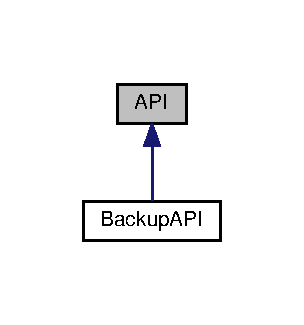
\includegraphics[width=146pt]{class_a_p_i__inherit__graph}
\end{center}
\end{figure}
\subsection*{Public Member Functions}
\begin{DoxyCompactItemize}
\item 
\hyperlink{class_a_p_i_af3ed2fc104249141ea1cca845bb80a5a}{\+\_\+\+\_\+construct} (\$request)
\item 
\mbox{\Hypertarget{class_a_p_i_a6469a4c34293f8aa7a4cf280147a4ab7}\label{class_a_p_i_a6469a4c34293f8aa7a4cf280147a4ab7}} 
{\bfseries process\+A\+PI} ()
\end{DoxyCompactItemize}
\subsection*{Protected Attributes}
\begin{DoxyCompactItemize}
\item 
\hyperlink{class_a_p_i_a5a9859ba17e15528c82f038a47eb3132}{\$method} = \textquotesingle{}\textquotesingle{}
\item 
\hyperlink{class_a_p_i_adabfc465b969f5dd4ec2c5f073e142ae}{\$endpoint} = \textquotesingle{}\textquotesingle{}
\item 
\hyperlink{class_a_p_i_a6a8f3d5321c4e9c7f3a9a29f0635b138}{\$verb} = \textquotesingle{}\textquotesingle{}
\item 
\hyperlink{class_a_p_i_a062ccad22e51e139ebf34d55abdb735d}{\$args} = Array()
\item 
\hyperlink{class_a_p_i_a045d1db08467e166b58c5af7447e02b4}{\$raw\+Data} = Null
\end{DoxyCompactItemize}


\subsection{Constructor \& Destructor Documentation}
\mbox{\Hypertarget{class_a_p_i_af3ed2fc104249141ea1cca845bb80a5a}\label{class_a_p_i_af3ed2fc104249141ea1cca845bb80a5a}} 
\index{A\+PI@{A\+PI}!\+\_\+\+\_\+construct@{\+\_\+\+\_\+construct}}
\index{\+\_\+\+\_\+construct@{\+\_\+\+\_\+construct}!A\+PI@{A\+PI}}
\subsubsection{\texorpdfstring{\+\_\+\+\_\+construct()}{\_\_construct()}}
{\footnotesize\ttfamily A\+P\+I\+::\+\_\+\+\_\+construct (\begin{DoxyParamCaption}\item[{}]{\$request }\end{DoxyParamCaption})}

Constructor\+: \+\_\+\+\_\+construct Allow for C\+O\+RS, assemble and pre-\/process the data 

\subsection{Member Data Documentation}
\mbox{\Hypertarget{class_a_p_i_a062ccad22e51e139ebf34d55abdb735d}\label{class_a_p_i_a062ccad22e51e139ebf34d55abdb735d}} 
\index{A\+PI@{A\+PI}!\$args@{\$args}}
\index{\$args@{\$args}!A\+PI@{A\+PI}}
\subsubsection{\texorpdfstring{\$args}{$args}}
{\footnotesize\ttfamily A\+P\+I\+::\$args = Array()\hspace{0.3cm}{\ttfamily [protected]}}

Property\+: args Any additional U\+RI components after the endpoint and verb have been removed, in our case, an integer ID for the resource. eg\+: /$<$endpoint$>$/$<$verb$>$/$<$arg0$>$/$<$arg1$>$ or /$<$endpoint$>$/$<$arg0$>$ \mbox{\Hypertarget{class_a_p_i_adabfc465b969f5dd4ec2c5f073e142ae}\label{class_a_p_i_adabfc465b969f5dd4ec2c5f073e142ae}} 
\index{A\+PI@{A\+PI}!\$endpoint@{\$endpoint}}
\index{\$endpoint@{\$endpoint}!A\+PI@{A\+PI}}
\subsubsection{\texorpdfstring{\$endpoint}{$endpoint}}
{\footnotesize\ttfamily A\+P\+I\+::\$endpoint = \textquotesingle{}\textquotesingle{}\hspace{0.3cm}{\ttfamily [protected]}}

Property\+: endpoint The Model requested in the U\+RI. eg\+: /files \mbox{\Hypertarget{class_a_p_i_a5a9859ba17e15528c82f038a47eb3132}\label{class_a_p_i_a5a9859ba17e15528c82f038a47eb3132}} 
\index{A\+PI@{A\+PI}!\$method@{\$method}}
\index{\$method@{\$method}!A\+PI@{A\+PI}}
\subsubsection{\texorpdfstring{\$method}{$method}}
{\footnotesize\ttfamily A\+P\+I\+::\$method = \textquotesingle{}\textquotesingle{}\hspace{0.3cm}{\ttfamily [protected]}}

Property\+: method The H\+T\+TP method this request was made in, either G\+ET, P\+O\+ST, P\+UT or D\+E\+L\+E\+TE \mbox{\Hypertarget{class_a_p_i_a045d1db08467e166b58c5af7447e02b4}\label{class_a_p_i_a045d1db08467e166b58c5af7447e02b4}} 
\index{A\+PI@{A\+PI}!\$raw\+Data@{\$raw\+Data}}
\index{\$raw\+Data@{\$raw\+Data}!A\+PI@{A\+PI}}
\subsubsection{\texorpdfstring{\$raw\+Data}{$rawData}}
{\footnotesize\ttfamily A\+P\+I\+::\$raw\+Data = Null\hspace{0.3cm}{\ttfamily [protected]}}

Property\+: raw\+Data Stores raw data from a P\+O\+ST or P\+UT \mbox{\Hypertarget{class_a_p_i_a6a8f3d5321c4e9c7f3a9a29f0635b138}\label{class_a_p_i_a6a8f3d5321c4e9c7f3a9a29f0635b138}} 
\index{A\+PI@{A\+PI}!\$verb@{\$verb}}
\index{\$verb@{\$verb}!A\+PI@{A\+PI}}
\subsubsection{\texorpdfstring{\$verb}{$verb}}
{\footnotesize\ttfamily A\+P\+I\+::\$verb = \textquotesingle{}\textquotesingle{}\hspace{0.3cm}{\ttfamily [protected]}}

Property\+: verb An optional additional descriptor about the endpoint, used for things that can not be handled by the basic methods. eg\+: /files/process 

The documentation for this class was generated from the following file\+:\begin{DoxyCompactItemize}
\item 
/home/kyle/cpp/bv-\/backup/server/http/core/api.\+class.\+php\end{DoxyCompactItemize}

\hypertarget{class_auth}{}\section{Auth Class Reference}
\label{class_auth}\index{Auth@{Auth}}


The documentation for this class was generated from the following file\+:\begin{DoxyCompactItemize}
\item 
/home/kyle/cpp/bv-\/backup/server/http/core/auth.\+class.\+php\end{DoxyCompactItemize}

\hypertarget{class_backup_a_p_i}{}\section{Backup\+A\+PI Class Reference}
\label{class_backup_a_p_i}\index{Backup\+A\+PI@{Backup\+A\+PI}}


Inheritance diagram for Backup\+A\+PI\+:
\nopagebreak
\begin{figure}[H]
\begin{center}
\leavevmode
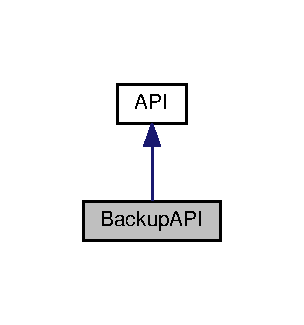
\includegraphics[width=146pt]{class_backup_a_p_i__inherit__graph}
\end{center}
\end{figure}


Collaboration diagram for Backup\+A\+PI\+:
\nopagebreak
\begin{figure}[H]
\begin{center}
\leavevmode
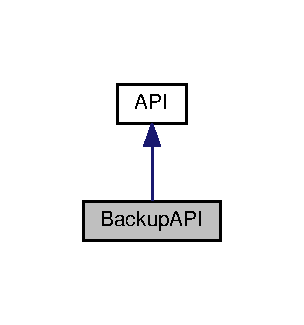
\includegraphics[width=146pt]{class_backup_a_p_i__coll__graph}
\end{center}
\end{figure}
\subsection*{Public Member Functions}
\begin{DoxyCompactItemize}
\item 
\mbox{\Hypertarget{class_backup_a_p_i_a4dcf5108de16dd3731ca7d455a436110}\label{class_backup_a_p_i_a4dcf5108de16dd3731ca7d455a436110}} 
{\bfseries \+\_\+\+\_\+construct} (\$request)
\end{DoxyCompactItemize}
\subsection*{Additional Inherited Members}


The documentation for this class was generated from the following file\+:\begin{DoxyCompactItemize}
\item 
/home/kyle/cpp/bv-\/backup/server/http/core/backup\+\_\+api.\+class.\+php\end{DoxyCompactItemize}

\hypertarget{class_backup_a_p_i_session}{}\section{Backup\+A\+P\+I\+Session Class Reference}
\label{class_backup_a_p_i_session}\index{Backup\+A\+P\+I\+Session@{Backup\+A\+P\+I\+Session}}
\subsection*{Public Member Functions}
\begin{DoxyCompactItemize}
\item 
\mbox{\Hypertarget{class_backup_a_p_i_session_a2eb66adcfe20654affe39015b851089a}\label{class_backup_a_p_i_session_a2eb66adcfe20654affe39015b851089a}} 
{\bfseries log\+Session} (\$endpoint, \$http\+\_\+method)
\item 
\mbox{\Hypertarget{class_backup_a_p_i_session_a986d734e555c33075911747d0f19be57}\label{class_backup_a_p_i_session_a986d734e555c33075911747d0f19be57}} 
{\bfseries is\+Authenticated} ()
\item 
\mbox{\Hypertarget{class_backup_a_p_i_session_a3fbe8aa59be9d0efe0dbd84e7db42d5a}\label{class_backup_a_p_i_session_a3fbe8aa59be9d0efe0dbd84e7db42d5a}} 
{\bfseries get\+User\+ID} ()
\end{DoxyCompactItemize}
\subsection*{Static Public Member Functions}
\begin{DoxyCompactItemize}
\item 
\mbox{\Hypertarget{class_backup_a_p_i_session_aacfebc7f42d2e17e6a66dd76b97c94ce}\label{class_backup_a_p_i_session_aacfebc7f42d2e17e6a66dd76b97c94ce}} 
static {\bfseries get\+Session} ()
\end{DoxyCompactItemize}


The documentation for this class was generated from the following file\+:\begin{DoxyCompactItemize}
\item 
/home/kyle/cpp/bv-\/backup/server/http/core/api\+\_\+session.\+class.\+php\end{DoxyCompactItemize}

\hypertarget{class_backup_database}{}\section{Backup\+Database Class Reference}
\label{class_backup_database}\index{Backup\+Database@{Backup\+Database}}
\subsection*{Public Member Functions}
\begin{DoxyCompactItemize}
\item 
\mbox{\Hypertarget{class_backup_database_a8f04f6cf7cf6c8a6635a5db3eb32a6f2}\label{class_backup_database_a8f04f6cf7cf6c8a6635a5db3eb32a6f2}} 
{\bfseries disconnect} ()
\item 
\mbox{\Hypertarget{class_backup_database_ae7c10f1130b39f2e77e2af4f2afa951d}\label{class_backup_database_ae7c10f1130b39f2e77e2af4f2afa951d}} 
{\bfseries get\+Connection} ()
\item 
\mbox{\Hypertarget{class_backup_database_ac9cf2430e87d8cbd7ec296c1f505e1a4}\label{class_backup_database_ac9cf2430e87d8cbd7ec296c1f505e1a4}} 
{\bfseries get\+Setting} (\$name)
\end{DoxyCompactItemize}
\subsection*{Static Public Member Functions}
\begin{DoxyCompactItemize}
\item 
\mbox{\Hypertarget{class_backup_database_a585876172d15c944234f9c1e47a3840b}\label{class_backup_database_a585876172d15c944234f9c1e47a3840b}} 
static {\bfseries get\+Database} ()
\end{DoxyCompactItemize}


The documentation for this class was generated from the following file\+:\begin{DoxyCompactItemize}
\item 
/home/kyle/cpp/bv-\/backup/server/http/core/database.\+class.\+php\end{DoxyCompactItemize}

\hypertarget{class_backup_1_1_file_1_1_backup_file}{}\section{Backup\+:\+:File\+:\+:Backup\+File Class Reference}
\label{class_backup_1_1_file_1_1_backup_file}\index{Backup\+::\+File\+::\+Backup\+File@{Backup\+::\+File\+::\+Backup\+File}}
\subsection*{Public Member Functions}
\begin{DoxyCompactItemize}
\item 
\mbox{\Hypertarget{class_backup_1_1_file_1_1_backup_file_a37c47e5e9c67cff51820f8f1cb3ea9f7}\label{class_backup_1_1_file_1_1_backup_file_a37c47e5e9c67cff51820f8f1cb3ea9f7}} 
{\bfseries Backup\+File} (const std\+::string \&file\+\_\+path)
\item 
\mbox{\Hypertarget{class_backup_1_1_file_1_1_backup_file_aa74000b82da3e8e3ba33fb6e65f20f97}\label{class_backup_1_1_file_1_1_backup_file_aa74000b82da3e8e3ba33fb6e65f20f97}} 
{\bfseries Backup\+File} (const fs\+::path \&file\+\_\+path)
\item 
\mbox{\Hypertarget{class_backup_1_1_file_1_1_backup_file_a2077b929aa3febb26717a810ce76d395}\label{class_backup_1_1_file_1_1_backup_file_a2077b929aa3febb26717a810ce76d395}} 
void \hyperlink{class_backup_1_1_file_1_1_backup_file_a2077b929aa3febb26717a810ce76d395}{set\+\_\+path} (const std\+::string \&fp)
\begin{DoxyCompactList}\small\item\em Assigns a new file path to the object. Setting the path triggers all of the associated member attributes and variables to be updated with private method update\+\_\+attributes() \end{DoxyCompactList}\item 
\mbox{\Hypertarget{class_backup_1_1_file_1_1_backup_file_a609874f97eb91023313e8fda7b8edb64}\label{class_backup_1_1_file_1_1_backup_file_a609874f97eb91023313e8fda7b8edb64}} 
void \hyperlink{class_backup_1_1_file_1_1_backup_file_a609874f97eb91023313e8fda7b8edb64}{set\+\_\+path} (const fs\+::path \&file\+\_\+path)
\begin{DoxyCompactList}\small\item\em Assigns a new file path to the object. Setting the path triggers all of the associated member attributes and variables to be updated with private method update\+\_\+attributes() \end{DoxyCompactList}\item 
\mbox{\Hypertarget{class_backup_1_1_file_1_1_backup_file_ac2b2bd4f4505e52368a2f4200a8795fa}\label{class_backup_1_1_file_1_1_backup_file_ac2b2bd4f4505e52368a2f4200a8795fa}} 
std\+::string {\bfseries get\+\_\+file\+\_\+name} () const
\item 
std\+::string \& \hyperlink{class_backup_1_1_file_1_1_backup_file_a0c5a9b6169c5724e97904de8b1f6c95c}{get\+\_\+file\+\_\+name} ()
\item 
size\+\_\+t \hyperlink{class_backup_1_1_file_1_1_backup_file_a482909cefc3cf777657a2500a7fd8c47}{get\+\_\+file\+\_\+size} ()
\item 
\mbox{\Hypertarget{class_backup_1_1_file_1_1_backup_file_af258fa0452d1ab95c69786e8c0516466}\label{class_backup_1_1_file_1_1_backup_file_af258fa0452d1ab95c69786e8c0516466}} 
std\+::string {\bfseries get\+\_\+file\+\_\+type} () const
\item 
std\+::string \& \hyperlink{class_backup_1_1_file_1_1_backup_file_abc2a8b1743ceb5b1ce8a7a9ce7967804}{get\+\_\+file\+\_\+type} ()
\item 
\mbox{\Hypertarget{class_backup_1_1_file_1_1_backup_file_a168de9c6391d4424e5b61f7813bdddbf}\label{class_backup_1_1_file_1_1_backup_file_a168de9c6391d4424e5b61f7813bdddbf}} 
std\+::string {\bfseries get\+\_\+unique\+\_\+id} () const
\item 
std\+::string \& \hyperlink{class_backup_1_1_file_1_1_backup_file_adc5feacc7ab47c0761b807c389bdef86}{get\+\_\+unique\+\_\+id} ()
\item 
std\+::string \hyperlink{class_backup_1_1_file_1_1_backup_file_ac799d37d7332c16e10c660123dadc30a}{get\+\_\+hash} (bool use\+\_\+file\+\_\+source=false)
\item 
unsigned int \hyperlink{class_backup_1_1_file_1_1_backup_file_ada76c8701596d88b1c12fefe7687c5b4}{get\+\_\+directory\+\_\+id} ()
\item 
\mbox{\Hypertarget{class_backup_1_1_file_1_1_backup_file_a656f2a4a6b59de41c9cc5135cbe0909f}\label{class_backup_1_1_file_1_1_backup_file_a656f2a4a6b59de41c9cc5135cbe0909f}} 
void \hyperlink{class_backup_1_1_file_1_1_backup_file_a656f2a4a6b59de41c9cc5135cbe0909f}{set\+\_\+directory\+\_\+id} (unsigned int id)
\begin{DoxyCompactList}\small\item\em Sets the associated database directory ID for the file (object only) \end{DoxyCompactList}\item 
unsigned int \hyperlink{class_backup_1_1_file_1_1_backup_file_a53e76e663bc651d68cfa9010788fee99}{get\+\_\+file\+\_\+id} ()
\item 
\mbox{\Hypertarget{class_backup_1_1_file_1_1_backup_file_af6e942ac6788f1793c9e530ce0e6dd0e}\label{class_backup_1_1_file_1_1_backup_file_af6e942ac6788f1793c9e530ce0e6dd0e}} 
void \hyperlink{class_backup_1_1_file_1_1_backup_file_af6e942ac6788f1793c9e530ce0e6dd0e}{set\+\_\+file\+\_\+id} (unsigned int id)
\begin{DoxyCompactList}\small\item\em Sets the associated database file ID for the file (object only) \end{DoxyCompactList}\item 
std\+::string \hyperlink{class_backup_1_1_file_1_1_backup_file_adad544ac9e93f4f45d1e1b56f7b2abc7}{get\+\_\+file\+\_\+path} () const
\item 
std\+::string \& \hyperlink{class_backup_1_1_file_1_1_backup_file_af0c9761572152255eb0e8ad6a99f7c91}{get\+\_\+file\+\_\+path} ()
\item 
std\+::string \hyperlink{class_backup_1_1_file_1_1_backup_file_a0131847a659a205885c5d6bfe324279d}{get\+\_\+parent\+\_\+path} () const
\item 
std\+::string \& \hyperlink{class_backup_1_1_file_1_1_backup_file_a2fd027d95d6e10aac23379989b78852b}{get\+\_\+parent\+\_\+path} ()
\item 
std\+::string \hyperlink{class_backup_1_1_file_1_1_backup_file_a1062ef23e1453ee672b7462b38fe76f7}{get\+\_\+relative\+\_\+path} () const
\item 
std\+::string \& \hyperlink{class_backup_1_1_file_1_1_backup_file_ac121d19028b1b5e95736e4416c73d6e3}{get\+\_\+relative\+\_\+path} ()
\item 
unsigned long \hyperlink{class_backup_1_1_file_1_1_backup_file_a2843c00b113857cc49f7494dab6f97b2}{get\+\_\+last\+\_\+modified} ()
\item 
bool \hyperlink{class_backup_1_1_file_1_1_backup_file_aed1719ae2bca1a1253956b4fd62a3383}{exists} ()
\item 
\mbox{\Hypertarget{class_backup_1_1_file_1_1_backup_file_a0556ed7ff0c08953d70398c83966892e}\label{class_backup_1_1_file_1_1_backup_file_a0556ed7ff0c08953d70398c83966892e}} 
bool {\bfseries is\+\_\+compressed} ()
\end{DoxyCompactItemize}


\subsection{Member Function Documentation}
\mbox{\Hypertarget{class_backup_1_1_file_1_1_backup_file_aed1719ae2bca1a1253956b4fd62a3383}\label{class_backup_1_1_file_1_1_backup_file_aed1719ae2bca1a1253956b4fd62a3383}} 
\index{Backup\+::\+File\+::\+Backup\+File@{Backup\+::\+File\+::\+Backup\+File}!exists@{exists}}
\index{exists@{exists}!Backup\+::\+File\+::\+Backup\+File@{Backup\+::\+File\+::\+Backup\+File}}
\subsubsection{\texorpdfstring{exists()}{exists()}}
{\footnotesize\ttfamily bool Backup\+File\+::exists (\begin{DoxyParamCaption}{ }\end{DoxyParamCaption})}

\begin{DoxyReturn}{Returns}
Returns whether or not the file exists 
\end{DoxyReturn}
\mbox{\Hypertarget{class_backup_1_1_file_1_1_backup_file_ada76c8701596d88b1c12fefe7687c5b4}\label{class_backup_1_1_file_1_1_backup_file_ada76c8701596d88b1c12fefe7687c5b4}} 
\index{Backup\+::\+File\+::\+Backup\+File@{Backup\+::\+File\+::\+Backup\+File}!get\+\_\+directory\+\_\+id@{get\+\_\+directory\+\_\+id}}
\index{get\+\_\+directory\+\_\+id@{get\+\_\+directory\+\_\+id}!Backup\+::\+File\+::\+Backup\+File@{Backup\+::\+File\+::\+Backup\+File}}
\subsubsection{\texorpdfstring{get\+\_\+directory\+\_\+id()}{get\_directory\_id()}}
{\footnotesize\ttfamily unsigned int Backup\+File\+::get\+\_\+directory\+\_\+id (\begin{DoxyParamCaption}{ }\end{DoxyParamCaption})}

\begin{DoxyReturn}{Returns}
Returns the database ID of the directory 
\end{DoxyReturn}
\mbox{\Hypertarget{class_backup_1_1_file_1_1_backup_file_a53e76e663bc651d68cfa9010788fee99}\label{class_backup_1_1_file_1_1_backup_file_a53e76e663bc651d68cfa9010788fee99}} 
\index{Backup\+::\+File\+::\+Backup\+File@{Backup\+::\+File\+::\+Backup\+File}!get\+\_\+file\+\_\+id@{get\+\_\+file\+\_\+id}}
\index{get\+\_\+file\+\_\+id@{get\+\_\+file\+\_\+id}!Backup\+::\+File\+::\+Backup\+File@{Backup\+::\+File\+::\+Backup\+File}}
\subsubsection{\texorpdfstring{get\+\_\+file\+\_\+id()}{get\_file\_id()}}
{\footnotesize\ttfamily unsigned int Backup\+File\+::get\+\_\+file\+\_\+id (\begin{DoxyParamCaption}{ }\end{DoxyParamCaption})}

\begin{DoxyReturn}{Returns}
Returns the database ID of the file 
\end{DoxyReturn}
\mbox{\Hypertarget{class_backup_1_1_file_1_1_backup_file_a0c5a9b6169c5724e97904de8b1f6c95c}\label{class_backup_1_1_file_1_1_backup_file_a0c5a9b6169c5724e97904de8b1f6c95c}} 
\index{Backup\+::\+File\+::\+Backup\+File@{Backup\+::\+File\+::\+Backup\+File}!get\+\_\+file\+\_\+name@{get\+\_\+file\+\_\+name}}
\index{get\+\_\+file\+\_\+name@{get\+\_\+file\+\_\+name}!Backup\+::\+File\+::\+Backup\+File@{Backup\+::\+File\+::\+Backup\+File}}
\subsubsection{\texorpdfstring{get\+\_\+file\+\_\+name()}{get\_file\_name()}}
{\footnotesize\ttfamily std\+::string Backup\+File\+::get\+\_\+file\+\_\+name (\begin{DoxyParamCaption}{ }\end{DoxyParamCaption})}

\begin{DoxyReturn}{Returns}
Returns the filename 
\end{DoxyReturn}
\mbox{\Hypertarget{class_backup_1_1_file_1_1_backup_file_adad544ac9e93f4f45d1e1b56f7b2abc7}\label{class_backup_1_1_file_1_1_backup_file_adad544ac9e93f4f45d1e1b56f7b2abc7}} 
\index{Backup\+::\+File\+::\+Backup\+File@{Backup\+::\+File\+::\+Backup\+File}!get\+\_\+file\+\_\+path@{get\+\_\+file\+\_\+path}}
\index{get\+\_\+file\+\_\+path@{get\+\_\+file\+\_\+path}!Backup\+::\+File\+::\+Backup\+File@{Backup\+::\+File\+::\+Backup\+File}}
\subsubsection{\texorpdfstring{get\+\_\+file\+\_\+path()}{get\_file\_path()}\hspace{0.1cm}{\footnotesize\ttfamily [1/2]}}
{\footnotesize\ttfamily std\+::string Backup\+File\+::get\+\_\+file\+\_\+path (\begin{DoxyParamCaption}{ }\end{DoxyParamCaption}) const}

\begin{DoxyReturn}{Returns}
Returns the complete file path as a string 
\end{DoxyReturn}
\mbox{\Hypertarget{class_backup_1_1_file_1_1_backup_file_af0c9761572152255eb0e8ad6a99f7c91}\label{class_backup_1_1_file_1_1_backup_file_af0c9761572152255eb0e8ad6a99f7c91}} 
\index{Backup\+::\+File\+::\+Backup\+File@{Backup\+::\+File\+::\+Backup\+File}!get\+\_\+file\+\_\+path@{get\+\_\+file\+\_\+path}}
\index{get\+\_\+file\+\_\+path@{get\+\_\+file\+\_\+path}!Backup\+::\+File\+::\+Backup\+File@{Backup\+::\+File\+::\+Backup\+File}}
\subsubsection{\texorpdfstring{get\+\_\+file\+\_\+path()}{get\_file\_path()}\hspace{0.1cm}{\footnotesize\ttfamily [2/2]}}
{\footnotesize\ttfamily std\+::string \& Backup\+File\+::get\+\_\+file\+\_\+path (\begin{DoxyParamCaption}{ }\end{DoxyParamCaption})}

\begin{DoxyReturn}{Returns}
Returns the complete file path as a string 
\end{DoxyReturn}
\mbox{\Hypertarget{class_backup_1_1_file_1_1_backup_file_a482909cefc3cf777657a2500a7fd8c47}\label{class_backup_1_1_file_1_1_backup_file_a482909cefc3cf777657a2500a7fd8c47}} 
\index{Backup\+::\+File\+::\+Backup\+File@{Backup\+::\+File\+::\+Backup\+File}!get\+\_\+file\+\_\+size@{get\+\_\+file\+\_\+size}}
\index{get\+\_\+file\+\_\+size@{get\+\_\+file\+\_\+size}!Backup\+::\+File\+::\+Backup\+File@{Backup\+::\+File\+::\+Backup\+File}}
\subsubsection{\texorpdfstring{get\+\_\+file\+\_\+size()}{get\_file\_size()}}
{\footnotesize\ttfamily size\+\_\+t Backup\+File\+::get\+\_\+file\+\_\+size (\begin{DoxyParamCaption}{ }\end{DoxyParamCaption})}

\begin{DoxyReturn}{Returns}
Returns the file size 
\end{DoxyReturn}
\mbox{\Hypertarget{class_backup_1_1_file_1_1_backup_file_abc2a8b1743ceb5b1ce8a7a9ce7967804}\label{class_backup_1_1_file_1_1_backup_file_abc2a8b1743ceb5b1ce8a7a9ce7967804}} 
\index{Backup\+::\+File\+::\+Backup\+File@{Backup\+::\+File\+::\+Backup\+File}!get\+\_\+file\+\_\+type@{get\+\_\+file\+\_\+type}}
\index{get\+\_\+file\+\_\+type@{get\+\_\+file\+\_\+type}!Backup\+::\+File\+::\+Backup\+File@{Backup\+::\+File\+::\+Backup\+File}}
\subsubsection{\texorpdfstring{get\+\_\+file\+\_\+type()}{get\_file\_type()}}
{\footnotesize\ttfamily std\+::string Backup\+File\+::get\+\_\+file\+\_\+type (\begin{DoxyParamCaption}{ }\end{DoxyParamCaption})}

\begin{DoxyReturn}{Returns}
Returns the file extension as a string 
\end{DoxyReturn}
\mbox{\Hypertarget{class_backup_1_1_file_1_1_backup_file_ac799d37d7332c16e10c660123dadc30a}\label{class_backup_1_1_file_1_1_backup_file_ac799d37d7332c16e10c660123dadc30a}} 
\index{Backup\+::\+File\+::\+Backup\+File@{Backup\+::\+File\+::\+Backup\+File}!get\+\_\+hash@{get\+\_\+hash}}
\index{get\+\_\+hash@{get\+\_\+hash}!Backup\+::\+File\+::\+Backup\+File@{Backup\+::\+File\+::\+Backup\+File}}
\subsubsection{\texorpdfstring{get\+\_\+hash()}{get\_hash()}}
{\footnotesize\ttfamily std\+::string Backup\+File\+::get\+\_\+hash (\begin{DoxyParamCaption}\item[{bool}]{use\+\_\+file\+\_\+source = {\ttfamily false} }\end{DoxyParamCaption})}

\begin{DoxyReturn}{Returns}
Returns a S\+H\+A-\/1 hash of the file contents 
\end{DoxyReturn}

\begin{DoxyParams}{Parameters}
{\em use\+\_\+file\+\_\+source} & Use Crypto\+PP File\+Source class vs. String\+Source (default=false) \\
\hline
\end{DoxyParams}
This peforms about 20\% slower than reading the file manually and passing to String\+Source\mbox{\Hypertarget{class_backup_1_1_file_1_1_backup_file_a2843c00b113857cc49f7494dab6f97b2}\label{class_backup_1_1_file_1_1_backup_file_a2843c00b113857cc49f7494dab6f97b2}} 
\index{Backup\+::\+File\+::\+Backup\+File@{Backup\+::\+File\+::\+Backup\+File}!get\+\_\+last\+\_\+modified@{get\+\_\+last\+\_\+modified}}
\index{get\+\_\+last\+\_\+modified@{get\+\_\+last\+\_\+modified}!Backup\+::\+File\+::\+Backup\+File@{Backup\+::\+File\+::\+Backup\+File}}
\subsubsection{\texorpdfstring{get\+\_\+last\+\_\+modified()}{get\_last\_modified()}}
{\footnotesize\ttfamily unsigned long Backup\+File\+::get\+\_\+last\+\_\+modified (\begin{DoxyParamCaption}{ }\end{DoxyParamCaption})}

\begin{DoxyReturn}{Returns}
Returns the last write time of the file as a Unix timestamp 
\end{DoxyReturn}
\mbox{\Hypertarget{class_backup_1_1_file_1_1_backup_file_a0131847a659a205885c5d6bfe324279d}\label{class_backup_1_1_file_1_1_backup_file_a0131847a659a205885c5d6bfe324279d}} 
\index{Backup\+::\+File\+::\+Backup\+File@{Backup\+::\+File\+::\+Backup\+File}!get\+\_\+parent\+\_\+path@{get\+\_\+parent\+\_\+path}}
\index{get\+\_\+parent\+\_\+path@{get\+\_\+parent\+\_\+path}!Backup\+::\+File\+::\+Backup\+File@{Backup\+::\+File\+::\+Backup\+File}}
\subsubsection{\texorpdfstring{get\+\_\+parent\+\_\+path()}{get\_parent\_path()}\hspace{0.1cm}{\footnotesize\ttfamily [1/2]}}
{\footnotesize\ttfamily std\+::string Backup\+File\+::get\+\_\+parent\+\_\+path (\begin{DoxyParamCaption}{ }\end{DoxyParamCaption}) const}

\begin{DoxyReturn}{Returns}
Returns the parent path of the file as a string 
\end{DoxyReturn}
\mbox{\Hypertarget{class_backup_1_1_file_1_1_backup_file_a2fd027d95d6e10aac23379989b78852b}\label{class_backup_1_1_file_1_1_backup_file_a2fd027d95d6e10aac23379989b78852b}} 
\index{Backup\+::\+File\+::\+Backup\+File@{Backup\+::\+File\+::\+Backup\+File}!get\+\_\+parent\+\_\+path@{get\+\_\+parent\+\_\+path}}
\index{get\+\_\+parent\+\_\+path@{get\+\_\+parent\+\_\+path}!Backup\+::\+File\+::\+Backup\+File@{Backup\+::\+File\+::\+Backup\+File}}
\subsubsection{\texorpdfstring{get\+\_\+parent\+\_\+path()}{get\_parent\_path()}\hspace{0.1cm}{\footnotesize\ttfamily [2/2]}}
{\footnotesize\ttfamily std\+::string \& Backup\+File\+::get\+\_\+parent\+\_\+path (\begin{DoxyParamCaption}{ }\end{DoxyParamCaption})}

\begin{DoxyReturn}{Returns}
Returns the parent path of the file as a string 
\end{DoxyReturn}
\mbox{\Hypertarget{class_backup_1_1_file_1_1_backup_file_a1062ef23e1453ee672b7462b38fe76f7}\label{class_backup_1_1_file_1_1_backup_file_a1062ef23e1453ee672b7462b38fe76f7}} 
\index{Backup\+::\+File\+::\+Backup\+File@{Backup\+::\+File\+::\+Backup\+File}!get\+\_\+relative\+\_\+path@{get\+\_\+relative\+\_\+path}}
\index{get\+\_\+relative\+\_\+path@{get\+\_\+relative\+\_\+path}!Backup\+::\+File\+::\+Backup\+File@{Backup\+::\+File\+::\+Backup\+File}}
\subsubsection{\texorpdfstring{get\+\_\+relative\+\_\+path()}{get\_relative\_path()}\hspace{0.1cm}{\footnotesize\ttfamily [1/2]}}
{\footnotesize\ttfamily std\+::string Backup\+File\+::get\+\_\+relative\+\_\+path (\begin{DoxyParamCaption}{ }\end{DoxyParamCaption}) const}

\begin{DoxyReturn}{Returns}
Returns the relative path of the file as a string 
\end{DoxyReturn}
\mbox{\Hypertarget{class_backup_1_1_file_1_1_backup_file_ac121d19028b1b5e95736e4416c73d6e3}\label{class_backup_1_1_file_1_1_backup_file_ac121d19028b1b5e95736e4416c73d6e3}} 
\index{Backup\+::\+File\+::\+Backup\+File@{Backup\+::\+File\+::\+Backup\+File}!get\+\_\+relative\+\_\+path@{get\+\_\+relative\+\_\+path}}
\index{get\+\_\+relative\+\_\+path@{get\+\_\+relative\+\_\+path}!Backup\+::\+File\+::\+Backup\+File@{Backup\+::\+File\+::\+Backup\+File}}
\subsubsection{\texorpdfstring{get\+\_\+relative\+\_\+path()}{get\_relative\_path()}\hspace{0.1cm}{\footnotesize\ttfamily [2/2]}}
{\footnotesize\ttfamily std\+::string \& Backup\+File\+::get\+\_\+relative\+\_\+path (\begin{DoxyParamCaption}{ }\end{DoxyParamCaption})}

\begin{DoxyReturn}{Returns}
Returns the relative path of the file as a string 
\end{DoxyReturn}
\mbox{\Hypertarget{class_backup_1_1_file_1_1_backup_file_adc5feacc7ab47c0761b807c389bdef86}\label{class_backup_1_1_file_1_1_backup_file_adc5feacc7ab47c0761b807c389bdef86}} 
\index{Backup\+::\+File\+::\+Backup\+File@{Backup\+::\+File\+::\+Backup\+File}!get\+\_\+unique\+\_\+id@{get\+\_\+unique\+\_\+id}}
\index{get\+\_\+unique\+\_\+id@{get\+\_\+unique\+\_\+id}!Backup\+::\+File\+::\+Backup\+File@{Backup\+::\+File\+::\+Backup\+File}}
\subsubsection{\texorpdfstring{get\+\_\+unique\+\_\+id()}{get\_unique\_id()}}
{\footnotesize\ttfamily std\+::string Backup\+File\+::get\+\_\+unique\+\_\+id (\begin{DoxyParamCaption}{ }\end{DoxyParamCaption})}

\begin{DoxyReturn}{Returns}
Returns a S\+H\+A-\/1 hash of the file path 
\end{DoxyReturn}


The documentation for this class was generated from the following files\+:\begin{DoxyCompactItemize}
\item 
/home/kyle/cpp/bv-\/backup/core/file.\+hpp\item 
/home/kyle/cpp/bv-\/backup/core/file.\+cpp\end{DoxyCompactItemize}

\hypertarget{class_backup_file}{}\section{Backup\+File Class Reference}
\label{class_backup_file}\index{Backup\+File@{Backup\+File}}
\subsection*{Public Member Functions}
\begin{DoxyCompactItemize}
\item 
\mbox{\Hypertarget{class_backup_file_afb7310a4cdd9a7d338e38dc085c29dcf}\label{class_backup_file_afb7310a4cdd9a7d338e38dc085c29dcf}} 
{\bfseries \+\_\+\+\_\+construct} (\$file\+ID)
\item 
\mbox{\Hypertarget{class_backup_file_ad32c7a1f2a030009fb1eba67ee2818db}\label{class_backup_file_ad32c7a1f2a030009fb1eba67ee2818db}} 
{\bfseries get\+File} ()
\item 
\mbox{\Hypertarget{class_backup_file_ad8369ed74cf9d01c608092b99fe7a05b}\label{class_backup_file_ad8369ed74cf9d01c608092b99fe7a05b}} 
{\bfseries exists} ()
\end{DoxyCompactItemize}


The documentation for this class was generated from the following file\+:\begin{DoxyCompactItemize}
\item 
/home/kyle/cpp/bv-\/backup/server/http/core/file.\+class.\+php\end{DoxyCompactItemize}

\hypertarget{class_backup_l_d_a_p}{}\section{Backup\+L\+D\+AP Class Reference}
\label{class_backup_l_d_a_p}\index{Backup\+L\+D\+AP@{Backup\+L\+D\+AP}}
\subsection*{Public Member Functions}
\begin{DoxyCompactItemize}
\item 
\mbox{\Hypertarget{class_backup_l_d_a_p_a04cb372425b6cc6800a9a14f8bc55697}\label{class_backup_l_d_a_p_a04cb372425b6cc6800a9a14f8bc55697}} 
{\bfseries import\+Users} ()
\item 
\mbox{\Hypertarget{class_backup_l_d_a_p_a00034c4130b9d6b5c7c4a030b1436b80}\label{class_backup_l_d_a_p_a00034c4130b9d6b5c7c4a030b1436b80}} 
{\bfseries import\+Computers} ()
\end{DoxyCompactItemize}


The documentation for this class was generated from the following file\+:\begin{DoxyCompactItemize}
\item 
/home/kyle/cpp/bv-\/backup/server/http/core/ldap.\+class.\+php\end{DoxyCompactItemize}

\hypertarget{class_backup_log}{}\section{Backup\+Log Class Reference}
\label{class_backup_log}\index{Backup\+Log@{Backup\+Log}}
\subsection*{Public Member Functions}
\begin{DoxyCompactItemize}
\item 
\mbox{\Hypertarget{class_backup_log_aabfb60abae06cf690e5ccfc728105531}\label{class_backup_log_aabfb60abae06cf690e5ccfc728105531}} 
{\bfseries \+\_\+\+\_\+construct} (\$user\+ID)
\item 
\mbox{\Hypertarget{class_backup_log_acf30ac12c849476b251e00d3cd8353b1}\label{class_backup_log_acf30ac12c849476b251e00d3cd8353b1}} 
{\bfseries set\+User\+ID} (\$user\+ID)
\item 
\mbox{\Hypertarget{class_backup_log_a9ad64d907c5c454f4b26f4c130f8d489}\label{class_backup_log_a9ad64d907c5c454f4b26f4c130f8d489}} 
{\bfseries set\+Output} (\$flag)
\item 
\mbox{\Hypertarget{class_backup_log_aa053b23128c631fe63eeb41814cd1152}\label{class_backup_log_aa053b23128c631fe63eeb41814cd1152}} 
{\bfseries add\+Error} (\$msg, \$type=\textquotesingle{}Info\textquotesingle{}, \$priority=0, \$output=false)
\item 
\mbox{\Hypertarget{class_backup_log_acba0c600bb1357c82712cb14f63900f9}\label{class_backup_log_acba0c600bb1357c82712cb14f63900f9}} 
{\bfseries add\+Message} (\$msg, \$type=\textquotesingle{}Info\textquotesingle{}, \$priority=0, \$output=false, \$error=0)
\end{DoxyCompactItemize}
\subsection*{Static Public Member Functions}
\begin{DoxyCompactItemize}
\item 
\mbox{\Hypertarget{class_backup_log_a827500235e604611037af2368a5b4141}\label{class_backup_log_a827500235e604611037af2368a5b4141}} 
static {\bfseries get\+Log} (\$user\+ID)
\end{DoxyCompactItemize}


The documentation for this class was generated from the following file\+:\begin{DoxyCompactItemize}
\item 
/home/kyle/cpp/bv-\/backup/server/http/core/log.\+class.\+php\end{DoxyCompactItemize}

\hypertarget{class_backup_machine}{}\section{Backup\+Machine Class Reference}
\label{class_backup_machine}\index{Backup\+Machine@{Backup\+Machine}}
\subsection*{Public Member Functions}
\begin{DoxyCompactItemize}
\item 
\mbox{\Hypertarget{class_backup_machine_a8b0fa3d937601284fc8546dabc0f653e}\label{class_backup_machine_a8b0fa3d937601284fc8546dabc0f653e}} 
{\bfseries \+\_\+\+\_\+construct} (\$host\+ID)
\item 
\mbox{\Hypertarget{class_backup_machine_a08f03ec33aaaeb9acfeb06eff67180fe}\label{class_backup_machine_a08f03ec33aaaeb9acfeb06eff67180fe}} 
{\bfseries exists} ()
\item 
\mbox{\Hypertarget{class_backup_machine_a795a38b44aed0468c8a3e13da854e084}\label{class_backup_machine_a795a38b44aed0468c8a3e13da854e084}} 
{\bfseries get\+Data} (\$field)
\end{DoxyCompactItemize}


The documentation for this class was generated from the following file\+:\begin{DoxyCompactItemize}
\item 
/home/kyle/cpp/bv-\/backup/server/http/core/machine.\+class.\+php\end{DoxyCompactItemize}

\hypertarget{class_backup_session}{}\section{Backup\+Session Class Reference}
\label{class_backup_session}\index{Backup\+Session@{Backup\+Session}}
\subsection*{Public Member Functions}
\begin{DoxyCompactItemize}
\item 
\mbox{\Hypertarget{class_backup_session_acc6683cf8d786e59ec0eb13074d5d5b3}\label{class_backup_session_acc6683cf8d786e59ec0eb13074d5d5b3}} 
{\bfseries get\+I\+P\+Addr} ()
\item 
\mbox{\Hypertarget{class_backup_session_a7e66f81601af667694b0dcac50a23bd4}\label{class_backup_session_a7e66f81601af667694b0dcac50a23bd4}} 
{\bfseries login} (\$username, \$pwd)
\item 
\mbox{\Hypertarget{class_backup_session_af2a67ef17feca4126fde4608942e876a}\label{class_backup_session_af2a67ef17feca4126fde4608942e876a}} 
{\bfseries is\+Logged\+In} ()
\item 
\mbox{\Hypertarget{class_backup_session_a9cb794c8f32a359f938a10b994a3fdda}\label{class_backup_session_a9cb794c8f32a359f938a10b994a3fdda}} 
{\bfseries logout} ()
\item 
\mbox{\Hypertarget{class_backup_session_a150334dceffd7e3ae15988d4446651c8}\label{class_backup_session_a150334dceffd7e3ae15988d4446651c8}} 
{\bfseries get\+User\+ID} ()
\item 
\mbox{\Hypertarget{class_backup_session_af197e1253feabe45999efbae44c86625}\label{class_backup_session_af197e1253feabe45999efbae44c86625}} 
{\bfseries get\+Session\+ID} ()
\item 
\mbox{\Hypertarget{class_backup_session_a49f3431e36ecc6c77e6384519bdf91d3}\label{class_backup_session_a49f3431e36ecc6c77e6384519bdf91d3}} 
{\bfseries print\+Login\+Msg} ()
\item 
\mbox{\Hypertarget{class_backup_session_a1dde966fbace7c52d63c6e0d4da42bcf}\label{class_backup_session_a1dde966fbace7c52d63c6e0d4da42bcf}} 
{\bfseries get\+Referer\+U\+RL} ()
\end{DoxyCompactItemize}
\subsection*{Static Public Member Functions}
\begin{DoxyCompactItemize}
\item 
\mbox{\Hypertarget{class_backup_session_ade409e52ef17402c176b492d2d580079}\label{class_backup_session_ade409e52ef17402c176b492d2d580079}} 
static {\bfseries get\+Session} ()
\end{DoxyCompactItemize}


The documentation for this class was generated from the following file\+:\begin{DoxyCompactItemize}
\item 
/home/kyle/cpp/bv-\/backup/server/http/core/session.\+class.\+php\end{DoxyCompactItemize}

\hypertarget{class_backup_upload}{}\section{Backup\+Upload Class Reference}
\label{class_backup_upload}\index{Backup\+Upload@{Backup\+Upload}}
\subsection*{Public Member Functions}
\begin{DoxyCompactItemize}
\item 
\mbox{\Hypertarget{class_backup_upload_a6166d726b5e228afe6a20d11bc6d9070}\label{class_backup_upload_a6166d726b5e228afe6a20d11bc6d9070}} 
{\bfseries \+\_\+\+\_\+construct} (\$file\+Metadata, \&\$file\+Content)
\item 
\hyperlink{class_backup_upload_afb809d66480b6925a4d1905e3237b051}{upload} ()
\item 
\mbox{\Hypertarget{class_backup_upload_a84facdb1488cde866f017ac2112d9be4}\label{class_backup_upload_a84facdb1488cde866f017ac2112d9be4}} 
{\bfseries upload\+\_\+part} ()
\item 
\mbox{\Hypertarget{class_backup_upload_a6438f4537080690e795ea466d01fe217}\label{class_backup_upload_a6438f4537080690e795ea466d01fe217}} 
{\bfseries is\+Valid} ()
\item 
\mbox{\Hypertarget{class_backup_upload_a2eec48aad82f9f43687a92b47d6c48e6}\label{class_backup_upload_a2eec48aad82f9f43687a92b47d6c48e6}} 
{\bfseries get\+Error} ()
\item 
\mbox{\Hypertarget{class_backup_upload_a80397e68071a5d00683b7778f35f5a13}\label{class_backup_upload_a80397e68071a5d00683b7778f35f5a13}} 
{\bfseries get\+File\+ID} ()
\item 
\mbox{\Hypertarget{class_backup_upload_a25c99a2c6c6a51e29d6374eb2a69aa2e}\label{class_backup_upload_a25c99a2c6c6a51e29d6374eb2a69aa2e}} 
{\bfseries get\+Upload\+ID} ()
\end{DoxyCompactItemize}


\subsection{Member Function Documentation}
\mbox{\Hypertarget{class_backup_upload_afb809d66480b6925a4d1905e3237b051}\label{class_backup_upload_afb809d66480b6925a4d1905e3237b051}} 
\index{Backup\+Upload@{Backup\+Upload}!upload@{upload}}
\index{upload@{upload}!Backup\+Upload@{Backup\+Upload}}
\subsubsection{\texorpdfstring{upload()}{upload()}}
{\footnotesize\ttfamily Backup\+Upload\+::upload (\begin{DoxyParamCaption}{ }\end{DoxyParamCaption})}

For single file uploads 

The documentation for this class was generated from the following file\+:\begin{DoxyCompactItemize}
\item 
/home/kyle/cpp/bv-\/backup/server/http/core/upload.\+class.\+php\end{DoxyCompactItemize}

\hypertarget{class_backup_user}{}\section{Backup\+User Class Reference}
\label{class_backup_user}\index{Backup\+User@{Backup\+User}}
\subsection*{Public Member Functions}
\begin{DoxyCompactItemize}
\item 
\mbox{\Hypertarget{class_backup_user_aee2c42d1e5f3fc18d58d7ce20b04ff69}\label{class_backup_user_aee2c42d1e5f3fc18d58d7ce20b04ff69}} 
{\bfseries \+\_\+\+\_\+construct} (\$user\+ID)
\item 
\mbox{\Hypertarget{class_backup_user_af2e762eb04d550cb9ddf2211c5770103}\label{class_backup_user_af2e762eb04d550cb9ddf2211c5770103}} 
{\bfseries get\+User\+Data} (\$col)
\item 
\mbox{\Hypertarget{class_backup_user_a4b51fb52e703fafdee12f67a265ec019}\label{class_backup_user_a4b51fb52e703fafdee12f67a265ec019}} 
{\bfseries set\+Password} (\$pwd)
\item 
\mbox{\Hypertarget{class_backup_user_a5b637dd4f8c1621ff2be46ac3e7f6bf9}\label{class_backup_user_a5b637dd4f8c1621ff2be46ac3e7f6bf9}} 
{\bfseries create\+User\+Activation} (\$code=\textquotesingle{}\textquotesingle{})
\item 
\mbox{\Hypertarget{class_backup_user_a980f26c158e68188e940cc3c7f29c1f3}\label{class_backup_user_a980f26c158e68188e940cc3c7f29c1f3}} 
{\bfseries activate\+User} (\$activation\+Code)
\end{DoxyCompactItemize}
\subsection*{Static Public Member Functions}
\begin{DoxyCompactItemize}
\item 
\mbox{\Hypertarget{class_backup_user_a955a6e50598ece7d2a5bdf6f41bfbae4}\label{class_backup_user_a955a6e50598ece7d2a5bdf6f41bfbae4}} 
static {\bfseries get\+User} (\$user\+ID)
\item 
\mbox{\Hypertarget{class_backup_user_a816d22afa5eb3ef679d9e522eb5bc4c3}\label{class_backup_user_a816d22afa5eb3ef679d9e522eb5bc4c3}} 
static {\bfseries generate\+Access\+Token} ()
\item 
\mbox{\Hypertarget{class_backup_user_a4366d21e76920addcf9e92f4becb6701}\label{class_backup_user_a4366d21e76920addcf9e92f4becb6701}} 
static {\bfseries user\+Exists} (\$user\+Name)
\end{DoxyCompactItemize}


The documentation for this class was generated from the following file\+:\begin{DoxyCompactItemize}
\item 
/home/kyle/cpp/bv-\/backup/server/http/core/user.\+class.\+php\end{DoxyCompactItemize}

\hypertarget{class_backup_1_1_networking_1_1_client}{}\section{Backup\+:\+:Networking\+:\+:Client Class Reference}
\label{class_backup_1_1_networking_1_1_client}\index{Backup\+::\+Networking\+::\+Client@{Backup\+::\+Networking\+::\+Client}}
\subsection*{Public Member Functions}
\begin{DoxyCompactItemize}
\item 
\mbox{\Hypertarget{class_backup_1_1_networking_1_1_client_a787bea154370a9d165b0fa4f2a9340a1}\label{class_backup_1_1_networking_1_1_client_a787bea154370a9d165b0fa4f2a9340a1}} 
{\bfseries Client} (const std\+::string \&hostname)
\item 
\mbox{\Hypertarget{class_backup_1_1_networking_1_1_client_abccb976632db0b3b5df925875b80b2e7}\label{class_backup_1_1_networking_1_1_client_abccb976632db0b3b5df925875b80b2e7}} 
bool {\bfseries connect} ()
\item 
\mbox{\Hypertarget{class_backup_1_1_networking_1_1_client_a97e144b48409c0a9873eee09f04ce724}\label{class_backup_1_1_networking_1_1_client_a97e144b48409c0a9873eee09f04ce724}} 
void {\bfseries disconnect} ()
\item 
\mbox{\Hypertarget{class_backup_1_1_networking_1_1_client_a1654a80c5c715694b9ad5a8f7db8b6b0}\label{class_backup_1_1_networking_1_1_client_a1654a80c5c715694b9ad5a8f7db8b6b0}} 
bool {\bfseries is\+\_\+connected} ()
\item 
\mbox{\Hypertarget{class_backup_1_1_networking_1_1_client_a32bc5f8ee7fab0d86e86247a1a6a3d21}\label{class_backup_1_1_networking_1_1_client_a32bc5f8ee7fab0d86e86247a1a6a3d21}} 
void {\bfseries set\+\_\+timeout} (boost\+::posix\+\_\+time\+::time\+\_\+duration t)
\item 
\mbox{\Hypertarget{class_backup_1_1_networking_1_1_client_a414faccfe00dacbb75f4bdf92a531770}\label{class_backup_1_1_networking_1_1_client_a414faccfe00dacbb75f4bdf92a531770}} 
void {\bfseries set\+\_\+ssl} (bool f)
\item 
\mbox{\Hypertarget{class_backup_1_1_networking_1_1_client_a48973fb82474072290509dc6e7bd369a}\label{class_backup_1_1_networking_1_1_client_a48973fb82474072290509dc6e7bd369a}} 
void {\bfseries send\+\_\+request} (const \hyperlink{class_backup_1_1_networking_1_1_http_request}{Backup\+::\+Networking\+::\+Http\+Request} \&r)
\item 
\mbox{\Hypertarget{class_backup_1_1_networking_1_1_client_a2d4d14d6aeee19c25a2ae0f8fbb3387f}\label{class_backup_1_1_networking_1_1_client_a2d4d14d6aeee19c25a2ae0f8fbb3387f}} 
bool {\bfseries upload\+\_\+file\+\_\+single} (const \hyperlink{struct_backup_1_1_types_1_1http__upload__file}{Backup\+::\+Types\+::http\+\_\+upload\+\_\+file} \&f)
\item 
\mbox{\Hypertarget{class_backup_1_1_networking_1_1_client_a253927293aef3a3e27c1f1c2fdb4aeb7}\label{class_backup_1_1_networking_1_1_client_a253927293aef3a3e27c1f1c2fdb4aeb7}} 
bool {\bfseries upload\+\_\+file\+\_\+part} (const \hyperlink{struct_backup_1_1_types_1_1http__upload__file}{Backup\+::\+Types\+::http\+\_\+upload\+\_\+file} \&f)
\item 
\mbox{\Hypertarget{class_backup_1_1_networking_1_1_client_aa013e81c21518b1bf73ef34a299a282c}\label{class_backup_1_1_networking_1_1_client_aa013e81c21518b1bf73ef34a299a282c}} 
bool {\bfseries heartbeat} ()
\item 
\mbox{\Hypertarget{class_backup_1_1_networking_1_1_client_a3c266c525f57ff238d641c19e9d9d9b6}\label{class_backup_1_1_networking_1_1_client_a3c266c525f57ff238d641c19e9d9d9b6}} 
std\+::string {\bfseries get\+\_\+client\+\_\+settings} ()
\item 
\mbox{\Hypertarget{class_backup_1_1_networking_1_1_client_ab89fd778cf90c0fe6082bd632c1aa521}\label{class_backup_1_1_networking_1_1_client_ab89fd778cf90c0fe6082bd632c1aa521}} 
std\+::string {\bfseries get\+\_\+response} ()
\item 
\mbox{\Hypertarget{class_backup_1_1_networking_1_1_client_a3d505c1dd66a343dffb5ab80f27bce6b}\label{class_backup_1_1_networking_1_1_client_a3d505c1dd66a343dffb5ab80f27bce6b}} 
std\+::string {\bfseries get\+\_\+headers} ()
\item 
\mbox{\Hypertarget{class_backup_1_1_networking_1_1_client_a9180d4b04e4220fb348c324f1facc08d}\label{class_backup_1_1_networking_1_1_client_a9180d4b04e4220fb348c324f1facc08d}} 
unsigned int {\bfseries get\+\_\+http\+\_\+status} ()
\item 
\mbox{\Hypertarget{class_backup_1_1_networking_1_1_client_ac605aefd756b4d961552890d3b460711}\label{class_backup_1_1_networking_1_1_client_ac605aefd756b4d961552890d3b460711}} 
bool {\bfseries activate} ()
\item 
\mbox{\Hypertarget{class_backup_1_1_networking_1_1_client_a3a322f210d20ff14c4f7b64ae1019bf0}\label{class_backup_1_1_networking_1_1_client_a3a322f210d20ff14c4f7b64ae1019bf0}} 
bool {\bfseries is\+\_\+activated} ()
\item 
\mbox{\Hypertarget{class_backup_1_1_networking_1_1_client_acf76ef5dbe64c9b64b27fdc9275b3d4b}\label{class_backup_1_1_networking_1_1_client_acf76ef5dbe64c9b64b27fdc9275b3d4b}} 
bool {\bfseries resume\+\_\+transfer} ()
\end{DoxyCompactItemize}


The documentation for this class was generated from the following files\+:\begin{DoxyCompactItemize}
\item 
/home/kyle/cpp/bv-\/backup/client/client.\+hpp\item 
/home/kyle/cpp/bv-\/backup/client/client.\+cpp\end{DoxyCompactItemize}

\hypertarget{class_backup_1_1_compression_1_1_compressor}{}\section{Backup\+:\+:Compression\+:\+:Compressor Class Reference}
\label{class_backup_1_1_compression_1_1_compressor}\index{Backup\+::\+Compression\+::\+Compressor@{Backup\+::\+Compression\+::\+Compressor}}
\subsection*{Public Member Functions}
\begin{DoxyCompactItemize}
\item 
\mbox{\Hypertarget{class_backup_1_1_compression_1_1_compressor_a277957091c7b6829c974806fb7da9e0e}\label{class_backup_1_1_compression_1_1_compressor_a277957091c7b6829c974806fb7da9e0e}} 
std\+::string {\bfseries operator$<$$<$} (const std\+::string \&s)
\item 
\mbox{\Hypertarget{class_backup_1_1_compression_1_1_compressor_ab10bc34803c735c8907a3338f0e376b9}\label{class_backup_1_1_compression_1_1_compressor_ab10bc34803c735c8907a3338f0e376b9}} 
std\+::string {\bfseries operator$>$$>$} (const std\+::string \&s)
\item 
\mbox{\Hypertarget{class_backup_1_1_compression_1_1_compressor_a30c7b68f91188ac2fee25144273705c8}\label{class_backup_1_1_compression_1_1_compressor_a30c7b68f91188ac2fee25144273705c8}} 
void {\bfseries compress\+\_\+file} (const std\+::string \&in, const std\+::string \&out)
\item 
\mbox{\Hypertarget{class_backup_1_1_compression_1_1_compressor_aaa3defb5a9fb563228cf8c4327e0edf3}\label{class_backup_1_1_compression_1_1_compressor_aaa3defb5a9fb563228cf8c4327e0edf3}} 
void {\bfseries decompress\+\_\+file} (const std\+::string \&in, const std\+::string \&out)
\item 
\mbox{\Hypertarget{class_backup_1_1_compression_1_1_compressor_ac3aba7a7504c0cc36984bde1a08c3ca4}\label{class_backup_1_1_compression_1_1_compressor_ac3aba7a7504c0cc36984bde1a08c3ca4}} 
int {\bfseries start\+\_\+decompression} (size\+\_\+t len)
\item 
\mbox{\Hypertarget{class_backup_1_1_compression_1_1_compressor_a3b8d31244a69b302da80aaaa42cb755c}\label{class_backup_1_1_compression_1_1_compressor_a3b8d31244a69b302da80aaaa42cb755c}} 
void {\bfseries end\+\_\+decompression} ()
\item 
\mbox{\Hypertarget{class_backup_1_1_compression_1_1_compressor_aceea4cdde4be9e44b2b6e1367045b73c}\label{class_backup_1_1_compression_1_1_compressor_aceea4cdde4be9e44b2b6e1367045b73c}} 
void {\bfseries set\+\_\+z\+\_\+level} (int level)
\end{DoxyCompactItemize}


The documentation for this class was generated from the following files\+:\begin{DoxyCompactItemize}
\item 
/home/kyle/cpp/bv-\/backup/core/compress.\+hpp\item 
/home/kyle/cpp/bv-\/backup/core/compress.\+cpp\end{DoxyCompactItemize}

\hypertarget{class_backup_1_1_networking_1_1_connection}{}\section{Backup\+:\+:Networking\+:\+:Connection Class Reference}
\label{class_backup_1_1_networking_1_1_connection}\index{Backup\+::\+Networking\+::\+Connection@{Backup\+::\+Networking\+::\+Connection}}


Inheritance diagram for Backup\+:\+:Networking\+:\+:Connection\+:
\nopagebreak
\begin{figure}[H]
\begin{center}
\leavevmode
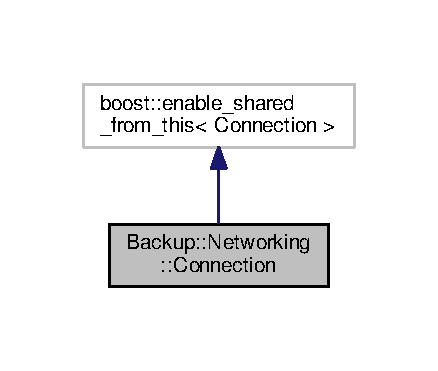
\includegraphics[width=210pt]{class_backup_1_1_networking_1_1_connection__inherit__graph}
\end{center}
\end{figure}


Collaboration diagram for Backup\+:\+:Networking\+:\+:Connection\+:
\nopagebreak
\begin{figure}[H]
\begin{center}
\leavevmode
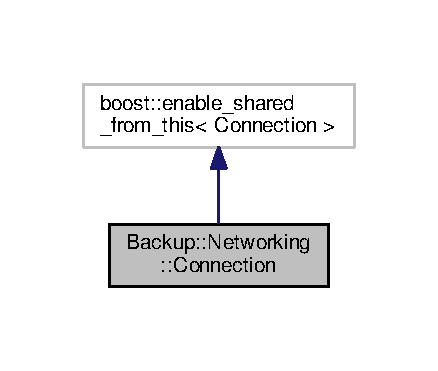
\includegraphics[width=210pt]{class_backup_1_1_networking_1_1_connection__coll__graph}
\end{center}
\end{figure}
\subsection*{Public Types}
\begin{DoxyCompactItemize}
\item 
\mbox{\Hypertarget{class_backup_1_1_networking_1_1_connection_a1b8db8cdf6210b8fb81ef1d5ae2411ba}\label{class_backup_1_1_networking_1_1_connection_a1b8db8cdf6210b8fb81ef1d5ae2411ba}} 
typedef boost\+::shared\+\_\+ptr$<$ \hyperlink{class_backup_1_1_networking_1_1_connection}{Connection} $>$ {\bfseries pointer}
\end{DoxyCompactItemize}
\subsection*{Public Member Functions}
\begin{DoxyCompactItemize}
\item 
\mbox{\Hypertarget{class_backup_1_1_networking_1_1_connection_a40dadb7d0b36d9359ef957eae9800876}\label{class_backup_1_1_networking_1_1_connection_a40dadb7d0b36d9359ef957eae9800876}} 
tcp\+::socket \& {\bfseries socket} ()
\item 
\mbox{\Hypertarget{class_backup_1_1_networking_1_1_connection_a47c25a31352a71e2a6902d37fc5fa2ba}\label{class_backup_1_1_networking_1_1_connection_a47c25a31352a71e2a6902d37fc5fa2ba}} 
void {\bfseries start} ()
\end{DoxyCompactItemize}
\subsection*{Static Public Member Functions}
\begin{DoxyCompactItemize}
\item 
\mbox{\Hypertarget{class_backup_1_1_networking_1_1_connection_a59b5460afc3e0637baedfaae94bb9a75}\label{class_backup_1_1_networking_1_1_connection_a59b5460afc3e0637baedfaae94bb9a75}} 
static pointer {\bfseries create} (boost\+::asio\+::io\+\_\+service \&io\+\_\+service)
\end{DoxyCompactItemize}


The documentation for this class was generated from the following files\+:\begin{DoxyCompactItemize}
\item 
/home/kyle/cpp/bv-\/backup/server/cpp/connection.\+hpp\item 
/home/kyle/cpp/bv-\/backup/server/cpp/connection.\+cpp\end{DoxyCompactItemize}

\hypertarget{struct_backup_1_1_types_1_1file__data}{}\section{Backup\+:\+:Types\+:\+:file\+\_\+data Struct Reference}
\label{struct_backup_1_1_types_1_1file__data}\index{Backup\+::\+Types\+::file\+\_\+data@{Backup\+::\+Types\+::file\+\_\+data}}
\subsection*{Public Attributes}
\begin{DoxyCompactItemize}
\item 
\mbox{\Hypertarget{struct_backup_1_1_types_1_1file__data_a37ab1cd69f26c8a3dab7fa68361324f6}\label{struct_backup_1_1_types_1_1file__data_a37ab1cd69f26c8a3dab7fa68361324f6}} 
std\+::string {\bfseries filename}
\item 
\mbox{\Hypertarget{struct_backup_1_1_types_1_1file__data_a2046deee135dcceb809bb9d6c1fd067f}\label{struct_backup_1_1_types_1_1file__data_a2046deee135dcceb809bb9d6c1fd067f}} 
std\+::string {\bfseries file\+\_\+ext}
\item 
\mbox{\Hypertarget{struct_backup_1_1_types_1_1file__data_a824d438a6dbb979fd43d5a3ab5baabf6}\label{struct_backup_1_1_types_1_1file__data_a824d438a6dbb979fd43d5a3ab5baabf6}} 
std\+::string {\bfseries parent\+\_\+path}
\item 
\mbox{\Hypertarget{struct_backup_1_1_types_1_1file__data_afb20032f61bd9aae6a82956961d7c01e}\label{struct_backup_1_1_types_1_1file__data_afb20032f61bd9aae6a82956961d7c01e}} 
size\+\_\+t {\bfseries filesize}
\item 
\mbox{\Hypertarget{struct_backup_1_1_types_1_1file__data_a966db7e9f839df95de076f0147afe6a7}\label{struct_backup_1_1_types_1_1file__data_a966db7e9f839df95de076f0147afe6a7}} 
size\+\_\+t {\bfseries compressed\+\_\+size}
\item 
\mbox{\Hypertarget{struct_backup_1_1_types_1_1file__data_a20455f1b6438496cfe080ae1292dba8d}\label{struct_backup_1_1_types_1_1file__data_a20455f1b6438496cfe080ae1292dba8d}} 
unsigned long {\bfseries last\+\_\+modified}
\item 
\mbox{\Hypertarget{struct_backup_1_1_types_1_1file__data_a5309ae239f26a2e631a67b84a7f74f1b}\label{struct_backup_1_1_types_1_1file__data_a5309ae239f26a2e631a67b84a7f74f1b}} 
unsigned int {\bfseries directory\+\_\+id}
\item 
\mbox{\Hypertarget{struct_backup_1_1_types_1_1file__data_a87b1dddbd6d13fd64db52e0b7e1f64b3}\label{struct_backup_1_1_types_1_1file__data_a87b1dddbd6d13fd64db52e0b7e1f64b3}} 
unsigned int {\bfseries file\+\_\+id}
\end{DoxyCompactItemize}


The documentation for this struct was generated from the following file\+:\begin{DoxyCompactItemize}
\item 
/home/kyle/cpp/bv-\/backup/core/types.\+hpp\end{DoxyCompactItemize}

\hypertarget{struct_backup_1_1_types_1_1file__directory}{}\section{Backup\+:\+:Types\+:\+:file\+\_\+directory Struct Reference}
\label{struct_backup_1_1_types_1_1file__directory}\index{Backup\+::\+Types\+::file\+\_\+directory@{Backup\+::\+Types\+::file\+\_\+directory}}
\subsection*{Public Attributes}
\begin{DoxyCompactItemize}
\item 
\mbox{\Hypertarget{struct_backup_1_1_types_1_1file__directory_a66d2b823b2c46ea4ed42fa1ec96460f9}\label{struct_backup_1_1_types_1_1file__directory_a66d2b823b2c46ea4ed42fa1ec96460f9}} 
std\+::string {\bfseries folder\+\_\+name}
\item 
\mbox{\Hypertarget{struct_backup_1_1_types_1_1file__directory_aa75499e15b9ebbc36af58b3315f80c50}\label{struct_backup_1_1_types_1_1file__directory_aa75499e15b9ebbc36af58b3315f80c50}} 
std\+::string {\bfseries path}
\item 
\mbox{\Hypertarget{struct_backup_1_1_types_1_1file__directory_af79f387cdfbba92ecbda5fb217ad03ed}\label{struct_backup_1_1_types_1_1file__directory_af79f387cdfbba92ecbda5fb217ad03ed}} 
unsigned int {\bfseries directory\+\_\+id}
\item 
\mbox{\Hypertarget{struct_backup_1_1_types_1_1file__directory_aa9fb09bc59cbff23f1123a27e76385f1}\label{struct_backup_1_1_types_1_1file__directory_aa9fb09bc59cbff23f1123a27e76385f1}} 
unsigned long {\bfseries last\+\_\+modified}
\item 
\mbox{\Hypertarget{struct_backup_1_1_types_1_1file__directory_a1c2072b7d87f918bd6d72bc005e293f9}\label{struct_backup_1_1_types_1_1file__directory_a1c2072b7d87f918bd6d72bc005e293f9}} 
size\+\_\+t {\bfseries filesize}
\end{DoxyCompactItemize}


The documentation for this struct was generated from the following file\+:\begin{DoxyCompactItemize}
\item 
/home/kyle/cpp/bv-\/backup/core/types.\+hpp\end{DoxyCompactItemize}

\hypertarget{class_backup_1_1_file_1_1_file_iterator}{}\section{Backup\+:\+:File\+:\+:File\+Iterator Class Reference}
\label{class_backup_1_1_file_1_1_file_iterator}\index{Backup\+::\+File\+::\+File\+Iterator@{Backup\+::\+File\+::\+File\+Iterator}}
\subsection*{Public Member Functions}
\begin{DoxyCompactItemize}
\item 
\mbox{\Hypertarget{class_backup_1_1_file_1_1_file_iterator_abd32f40496c43881fa9ad718e971b7cf}\label{class_backup_1_1_file_1_1_file_iterator_abd32f40496c43881fa9ad718e971b7cf}} 
{\bfseries File\+Iterator} (const std\+::string \&path)
\item 
\mbox{\Hypertarget{class_backup_1_1_file_1_1_file_iterator_ab98615126c4197146fd561621268ae0c}\label{class_backup_1_1_file_1_1_file_iterator_ab98615126c4197146fd561621268ae0c}} 
void {\bfseries scan} ()
\item 
\mbox{\Hypertarget{class_backup_1_1_file_1_1_file_iterator_a6dd7a72e190aeca2aab94149582e9e4e}\label{class_backup_1_1_file_1_1_file_iterator_a6dd7a72e190aeca2aab94149582e9e4e}} 
std\+::string {\bfseries get\+\_\+base\+\_\+path} ()
\end{DoxyCompactItemize}


The documentation for this class was generated from the following files\+:\begin{DoxyCompactItemize}
\item 
/home/kyle/cpp/bv-\/backup/core/file\+\_\+iterator.\+hpp\item 
/home/kyle/cpp/bv-\/backup/core/file\+\_\+iterator.\+cpp\end{DoxyCompactItemize}

\hypertarget{struct_backup_1_1_types_1_1http__request}{}\section{Backup\+:\+:Types\+:\+:http\+\_\+request Struct Reference}
\label{struct_backup_1_1_types_1_1http__request}\index{Backup\+::\+Types\+::http\+\_\+request@{Backup\+::\+Types\+::http\+\_\+request}}
\subsection*{Public Attributes}
\begin{DoxyCompactItemize}
\item 
\mbox{\Hypertarget{struct_backup_1_1_types_1_1http__request_ab67dede4a309e2db9f9aa671235a241d}\label{struct_backup_1_1_types_1_1http__request_ab67dede4a309e2db9f9aa671235a241d}} 
unsigned int {\bfseries request\+\_\+type}
\item 
\mbox{\Hypertarget{struct_backup_1_1_types_1_1http__request_a362e7fd66365d5f34ac63a50fcf65622}\label{struct_backup_1_1_types_1_1http__request_a362e7fd66365d5f34ac63a50fcf65622}} 
std\+::string {\bfseries uri}
\item 
\mbox{\Hypertarget{struct_backup_1_1_types_1_1http__request_a10ef0dae4190242fd60fc45d59ccc167}\label{struct_backup_1_1_types_1_1http__request_a10ef0dae4190242fd60fc45d59ccc167}} 
std\+::string {\bfseries content\+\_\+type}
\item 
\mbox{\Hypertarget{struct_backup_1_1_types_1_1http__request_a5ec6dfcfbbd5e9051d2a31e2576a0bce}\label{struct_backup_1_1_types_1_1http__request_a5ec6dfcfbbd5e9051d2a31e2576a0bce}} 
std\+::string {\bfseries data}
\item 
\mbox{\Hypertarget{struct_backup_1_1_types_1_1http__request_adff2e1766ef739fb3ad01d6fdaeb1585}\label{struct_backup_1_1_types_1_1http__request_adff2e1766ef739fb3ad01d6fdaeb1585}} 
std\+::string {\bfseries auth\+\_\+token}
\end{DoxyCompactItemize}


The documentation for this struct was generated from the following file\+:\begin{DoxyCompactItemize}
\item 
/home/kyle/cpp/bv-\/backup/core/types.\+hpp\end{DoxyCompactItemize}

\hypertarget{struct_backup_1_1_types_1_1http__upload__file}{}\section{Backup\+:\+:Types\+:\+:http\+\_\+upload\+\_\+file Struct Reference}
\label{struct_backup_1_1_types_1_1http__upload__file}\index{Backup\+::\+Types\+::http\+\_\+upload\+\_\+file@{Backup\+::\+Types\+::http\+\_\+upload\+\_\+file}}


Collaboration diagram for Backup\+:\+:Types\+:\+:http\+\_\+upload\+\_\+file\+:
\nopagebreak
\begin{figure}[H]
\begin{center}
\leavevmode
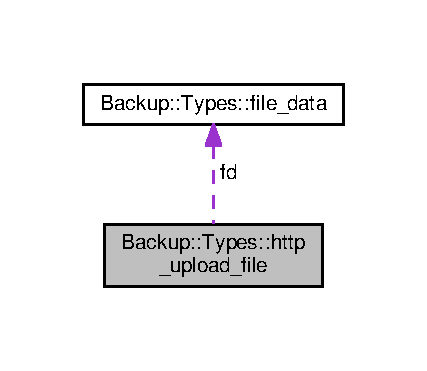
\includegraphics[width=205pt]{struct_backup_1_1_types_1_1http__upload__file__coll__graph}
\end{center}
\end{figure}
\subsection*{Public Attributes}
\begin{DoxyCompactItemize}
\item 
\mbox{\Hypertarget{struct_backup_1_1_types_1_1http__upload__file_a83e19aec410d33300bfb42f66f4ba402}\label{struct_backup_1_1_types_1_1http__upload__file_a83e19aec410d33300bfb42f66f4ba402}} 
\hyperlink{struct_backup_1_1_types_1_1file__data}{file\+\_\+data} {\bfseries fd}
\item 
\mbox{\Hypertarget{struct_backup_1_1_types_1_1http__upload__file_a0013011e56e720c81c8c3afb21a58d3f}\label{struct_backup_1_1_types_1_1http__upload__file_a0013011e56e720c81c8c3afb21a58d3f}} 
std\+::string {\bfseries file\+\_\+hash}
\item 
\mbox{\Hypertarget{struct_backup_1_1_types_1_1http__upload__file_a6ba75f5180113a22379cf998ce266339}\label{struct_backup_1_1_types_1_1http__upload__file_a6ba75f5180113a22379cf998ce266339}} 
std\+::string {\bfseries content}
\item 
\mbox{\Hypertarget{struct_backup_1_1_types_1_1http__upload__file_a73f312664509d364370a0072b9d77614}\label{struct_backup_1_1_types_1_1http__upload__file_a73f312664509d364370a0072b9d77614}} 
int {\bfseries part}
\item 
\mbox{\Hypertarget{struct_backup_1_1_types_1_1http__upload__file_ac5aa0823717adc9ca2510b0996a93484}\label{struct_backup_1_1_types_1_1http__upload__file_ac5aa0823717adc9ca2510b0996a93484}} 
int {\bfseries upload\+\_\+id}
\item 
\mbox{\Hypertarget{struct_backup_1_1_types_1_1http__upload__file_ae2a0eb51f4e154ab6b1203e71aff4b25}\label{struct_backup_1_1_types_1_1http__upload__file_ae2a0eb51f4e154ab6b1203e71aff4b25}} 
bool {\bfseries multi\+\_\+part}
\item 
\mbox{\Hypertarget{struct_backup_1_1_types_1_1http__upload__file_acea6776494bf00a3be9cc7535b0204d4}\label{struct_backup_1_1_types_1_1http__upload__file_acea6776494bf00a3be9cc7535b0204d4}} 
bool {\bfseries compressed}
\end{DoxyCompactItemize}


The documentation for this struct was generated from the following file\+:\begin{DoxyCompactItemize}
\item 
/home/kyle/cpp/bv-\/backup/core/types.\+hpp\end{DoxyCompactItemize}

\hypertarget{class_backup_1_1_networking_1_1_http_request}{}\section{Backup\+:\+:Networking\+:\+:Http\+Request Class Reference}
\label{class_backup_1_1_networking_1_1_http_request}\index{Backup\+::\+Networking\+::\+Http\+Request@{Backup\+::\+Networking\+::\+Http\+Request}}
\subsection*{Public Member Functions}
\begin{DoxyCompactItemize}
\item 
\mbox{\Hypertarget{class_backup_1_1_networking_1_1_http_request_a7e28f57fbabe252344e70cf634027796}\label{class_backup_1_1_networking_1_1_http_request_a7e28f57fbabe252344e70cf634027796}} 
void {\bfseries set\+\_\+uri} (const std\+::string \&str)
\item 
\mbox{\Hypertarget{class_backup_1_1_networking_1_1_http_request_a8f6d835d7fccdf697e34580107597345}\label{class_backup_1_1_networking_1_1_http_request_a8f6d835d7fccdf697e34580107597345}} 
void {\bfseries set\+\_\+method} (const std\+::string \&str)
\item 
\mbox{\Hypertarget{class_backup_1_1_networking_1_1_http_request_aec72630110b64ddc6d2b224371fa8905}\label{class_backup_1_1_networking_1_1_http_request_aec72630110b64ddc6d2b224371fa8905}} 
void {\bfseries add\+\_\+header} (const std\+::string \&str)
\item 
\mbox{\Hypertarget{class_backup_1_1_networking_1_1_http_request_a2aefa6612b6392f430727713fa0f7f72}\label{class_backup_1_1_networking_1_1_http_request_a2aefa6612b6392f430727713fa0f7f72}} 
void {\bfseries set\+\_\+content\+\_\+type} (const std\+::string \&str)
\item 
\mbox{\Hypertarget{class_backup_1_1_networking_1_1_http_request_a8bf38f9f7c70ed31fe1188dba372a486}\label{class_backup_1_1_networking_1_1_http_request_a8bf38f9f7c70ed31fe1188dba372a486}} 
void {\bfseries set\+\_\+body} (const std\+::string \&str)
\item 
\mbox{\Hypertarget{class_backup_1_1_networking_1_1_http_request_ac7898a1e392ea697272ddc147dbc6cbc}\label{class_backup_1_1_networking_1_1_http_request_ac7898a1e392ea697272ddc147dbc6cbc}} 
std\+::string {\bfseries get\+\_\+uri} () const
\item 
\mbox{\Hypertarget{class_backup_1_1_networking_1_1_http_request_aead79a239c592c8cdfe029dedbd25102}\label{class_backup_1_1_networking_1_1_http_request_aead79a239c592c8cdfe029dedbd25102}} 
std\+::string \& {\bfseries get\+\_\+uri} ()
\item 
\mbox{\Hypertarget{class_backup_1_1_networking_1_1_http_request_a546d7d55c73aaaed76d07e263fbf88f0}\label{class_backup_1_1_networking_1_1_http_request_a546d7d55c73aaaed76d07e263fbf88f0}} 
std\+::string {\bfseries get\+\_\+method} () const
\item 
\mbox{\Hypertarget{class_backup_1_1_networking_1_1_http_request_a09964b0dc7c35c994b98648057b11b8c}\label{class_backup_1_1_networking_1_1_http_request_a09964b0dc7c35c994b98648057b11b8c}} 
std\+::string \& {\bfseries get\+\_\+method} ()
\item 
\mbox{\Hypertarget{class_backup_1_1_networking_1_1_http_request_a8ced4962bba149da8febddce83a07148}\label{class_backup_1_1_networking_1_1_http_request_a8ced4962bba149da8febddce83a07148}} 
std\+::vector$<$ std\+::string $>$ \& {\bfseries get\+\_\+headers} ()
\item 
\mbox{\Hypertarget{class_backup_1_1_networking_1_1_http_request_a758a53c065a9ba07d12c87342cbf7488}\label{class_backup_1_1_networking_1_1_http_request_a758a53c065a9ba07d12c87342cbf7488}} 
std\+::vector$<$ std\+::string $>$ {\bfseries get\+\_\+headers} () const
\item 
\mbox{\Hypertarget{class_backup_1_1_networking_1_1_http_request_acdff7c432d22ac6ab7ce3eff63334ac7}\label{class_backup_1_1_networking_1_1_http_request_acdff7c432d22ac6ab7ce3eff63334ac7}} 
std\+::string \& {\bfseries get\+\_\+content\+\_\+type} ()
\item 
\mbox{\Hypertarget{class_backup_1_1_networking_1_1_http_request_a4c8063b3193e997a2bf958999055ea35}\label{class_backup_1_1_networking_1_1_http_request_a4c8063b3193e997a2bf958999055ea35}} 
std\+::string {\bfseries get\+\_\+content\+\_\+type} () const
\item 
\mbox{\Hypertarget{class_backup_1_1_networking_1_1_http_request_ac63afabbead609a3244dfe34518ee2b4}\label{class_backup_1_1_networking_1_1_http_request_ac63afabbead609a3244dfe34518ee2b4}} 
std\+::string \& {\bfseries get\+\_\+body} ()
\item 
\mbox{\Hypertarget{class_backup_1_1_networking_1_1_http_request_a77b5d51760c350a865e77c3bc0de3a42}\label{class_backup_1_1_networking_1_1_http_request_a77b5d51760c350a865e77c3bc0de3a42}} 
std\+::string {\bfseries get\+\_\+body} () const
\item 
\mbox{\Hypertarget{class_backup_1_1_networking_1_1_http_request_ab94815165bd2457bf4f8944ffc80148f}\label{class_backup_1_1_networking_1_1_http_request_ab94815165bd2457bf4f8944ffc80148f}} 
size\+\_\+t {\bfseries get\+\_\+body\+\_\+length} () const
\end{DoxyCompactItemize}


The documentation for this class was generated from the following files\+:\begin{DoxyCompactItemize}
\item 
/home/kyle/cpp/bv-\/backup/core/http\+\_\+request.\+hpp\item 
/home/kyle/cpp/bv-\/backup/core/http\+\_\+request.\+cpp\end{DoxyCompactItemize}

\hypertarget{class_backup_1_1_database_1_1_local_database}{}\section{Backup\+:\+:Database\+:\+:Local\+Database Class Reference}
\label{class_backup_1_1_database_1_1_local_database}\index{Backup\+::\+Database\+::\+Local\+Database@{Backup\+::\+Database\+::\+Local\+Database}}
\subsection*{Public Member Functions}
\begin{DoxyCompactItemize}
\item 
\mbox{\Hypertarget{class_backup_1_1_database_1_1_local_database_a5a1800d6a84e1ee09fb8ed03c1999d1a}\label{class_backup_1_1_database_1_1_local_database_a5a1800d6a84e1ee09fb8ed03c1999d1a}} 
{\bfseries Local\+Database} (\hyperlink{class_backup_1_1_database_1_1_local_database}{Local\+Database} const \&)=delete
\item 
\mbox{\Hypertarget{class_backup_1_1_database_1_1_local_database_a018b956b175c068c57958ae8b466e2bd}\label{class_backup_1_1_database_1_1_local_database_a018b956b175c068c57958ae8b466e2bd}} 
void {\bfseries operator=} (\hyperlink{class_backup_1_1_database_1_1_local_database}{Local\+Database} const \&)=delete
\item 
\mbox{\Hypertarget{class_backup_1_1_database_1_1_local_database_ab7bc1e783228e6413af275f1254d0c91}\label{class_backup_1_1_database_1_1_local_database_ab7bc1e783228e6413af275f1254d0c91}} 
bool {\bfseries is\+\_\+ignore\+\_\+dir} (const boost\+::filesystem\+::path \&p, int level)
\item 
\mbox{\Hypertarget{class_backup_1_1_database_1_1_local_database_a73d2320e6e1c3241f2b0dc8438c963e3}\label{class_backup_1_1_database_1_1_local_database_a73d2320e6e1c3241f2b0dc8438c963e3}} 
bool {\bfseries is\+\_\+ignore\+\_\+ext} (const std\+::string \&ext)
\item 
\mbox{\Hypertarget{class_backup_1_1_database_1_1_local_database_a9ebeda94ba4b1b981fa321ab2a60adb2}\label{class_backup_1_1_database_1_1_local_database_a9ebeda94ba4b1b981fa321ab2a60adb2}} 
std\+::string {\bfseries get\+\_\+setting\+\_\+str} (const std\+::string \&s)
\item 
\mbox{\Hypertarget{class_backup_1_1_database_1_1_local_database_aa7aa1872a73201ac03ebc6de375fd1d5}\label{class_backup_1_1_database_1_1_local_database_aa7aa1872a73201ac03ebc6de375fd1d5}} 
int {\bfseries get\+\_\+setting\+\_\+int} (const std\+::string \&s)
\item 
\mbox{\Hypertarget{class_backup_1_1_database_1_1_local_database_a7c6ac52eeb64f451d746ff3b3d3e3d3f}\label{class_backup_1_1_database_1_1_local_database_a7c6ac52eeb64f451d746ff3b3d3e3d3f}} 
{\footnotesize template$<$typename T $>$ }\\bool {\bfseries update\+\_\+setting} (const std\+::string \&key, const T \&val)
\item 
\mbox{\Hypertarget{class_backup_1_1_database_1_1_local_database_a18737407d07d0df8fd904061f139102b}\label{class_backup_1_1_database_1_1_local_database_a18737407d07d0df8fd904061f139102b}} 
bool {\bfseries update\+\_\+ext\+\_\+count} (const std\+::string \&ext, int total)
\item 
\mbox{\Hypertarget{class_backup_1_1_database_1_1_local_database_aeb27a45a2b956a5aa0f8ede9212ccc1c}\label{class_backup_1_1_database_1_1_local_database_aeb27a45a2b956a5aa0f8ede9212ccc1c}} 
unsigned int {\bfseries add\+\_\+file} (\hyperlink{class_backup_1_1_file_1_1_backup_file}{Backup\+::\+File\+::\+Backup\+File} $\ast$fd)
\item 
\mbox{\Hypertarget{class_backup_1_1_database_1_1_local_database_a3a03112d18428b1135a35c1b93aa6f50}\label{class_backup_1_1_database_1_1_local_database_a3a03112d18428b1135a35c1b93aa6f50}} 
unsigned int {\bfseries add\+\_\+directory} (\hyperlink{struct_backup_1_1_types_1_1file__directory}{Backup\+::\+Types\+::file\+\_\+directory} $\ast$fd)
\item 
\mbox{\Hypertarget{class_backup_1_1_database_1_1_local_database_aaf894e6e5b748b0c42701353f3741d0b}\label{class_backup_1_1_database_1_1_local_database_aaf894e6e5b748b0c42701353f3741d0b}} 
std\+::string {\bfseries get\+\_\+last\+\_\+err} ()
\item 
\mbox{\Hypertarget{class_backup_1_1_database_1_1_local_database_a1e3b91a1b4a4b3d54ff53ba82600abd3}\label{class_backup_1_1_database_1_1_local_database_a1e3b91a1b4a4b3d54ff53ba82600abd3}} 
void {\bfseries update\+\_\+global\+\_\+settings} ()
\item 
\mbox{\Hypertarget{class_backup_1_1_database_1_1_local_database_a27f71da48a1c85deda8b4651b3cc4eae}\label{class_backup_1_1_database_1_1_local_database_a27f71da48a1c85deda8b4651b3cc4eae}} 
void {\bfseries update\+\_\+client\+\_\+settings} (const std\+::string \&s)
\item 
\mbox{\Hypertarget{class_backup_1_1_database_1_1_local_database_a825296e65a28032e2ece0661c7d430a9}\label{class_backup_1_1_database_1_1_local_database_a825296e65a28032e2ece0661c7d430a9}} 
void {\bfseries clean} ()
\end{DoxyCompactItemize}
\subsection*{Static Public Member Functions}
\begin{DoxyCompactItemize}
\item 
\mbox{\Hypertarget{class_backup_1_1_database_1_1_local_database_a646eb6daa0b1fac43475137b351aa625}\label{class_backup_1_1_database_1_1_local_database_a646eb6daa0b1fac43475137b351aa625}} 
static \hyperlink{class_backup_1_1_database_1_1_local_database}{Local\+Database} \& {\bfseries get\+\_\+database} ()
\end{DoxyCompactItemize}


The documentation for this class was generated from the following files\+:\begin{DoxyCompactItemize}
\item 
/home/kyle/cpp/bv-\/backup/core/local\+\_\+db.\+hpp\item 
/home/kyle/cpp/bv-\/backup/core/local\+\_\+db.\+cpp\end{DoxyCompactItemize}

\hypertarget{class_backup_1_1_logging_1_1_log}{}\section{Backup\+:\+:Logging\+:\+:Log Class Reference}
\label{class_backup_1_1_logging_1_1_log}\index{Backup\+::\+Logging\+::\+Log@{Backup\+::\+Logging\+::\+Log}}
\subsection*{Public Member Functions}
\begin{DoxyCompactItemize}
\item 
\mbox{\Hypertarget{class_backup_1_1_logging_1_1_log_a06207517f314f71ccf7056e3a3ea100a}\label{class_backup_1_1_logging_1_1_log_a06207517f314f71ccf7056e3a3ea100a}} 
{\bfseries Log} (const std\+::string \&filename)
\item 
\mbox{\Hypertarget{class_backup_1_1_logging_1_1_log_a299f6114a1bcf2cd5b64018291bc8e3b}\label{class_backup_1_1_logging_1_1_log_a299f6114a1bcf2cd5b64018291bc8e3b}} 
void {\bfseries add\+\_\+message} (const std\+::string \&msg, const std\+::string \&category)
\item 
\mbox{\Hypertarget{class_backup_1_1_logging_1_1_log_a677c2bcb82015e0b75955a6736dda40a}\label{class_backup_1_1_logging_1_1_log_a677c2bcb82015e0b75955a6736dda40a}} 
void {\bfseries set\+\_\+level} (unsigned int level)
\end{DoxyCompactItemize}


The documentation for this class was generated from the following files\+:\begin{DoxyCompactItemize}
\item 
/home/kyle/cpp/bv-\/backup/core/log.\+hpp\item 
/home/kyle/cpp/bv-\/backup/core/log.\+cpp\end{DoxyCompactItemize}

\hypertarget{class_backup_1_1_networking_1_1_server}{}\section{Backup\+:\+:Networking\+:\+:Server Class Reference}
\label{class_backup_1_1_networking_1_1_server}\index{Backup\+::\+Networking\+::\+Server@{Backup\+::\+Networking\+::\+Server}}
\subsection*{Public Member Functions}
\begin{DoxyCompactItemize}
\item 
\mbox{\Hypertarget{class_backup_1_1_networking_1_1_server_ac9ad7c8bb7fe2f5da5101da1297c9ae1}\label{class_backup_1_1_networking_1_1_server_ac9ad7c8bb7fe2f5da5101da1297c9ae1}} 
{\bfseries Server} (boost\+::asio\+::io\+\_\+service \&io\+\_\+service)
\end{DoxyCompactItemize}


The documentation for this class was generated from the following files\+:\begin{DoxyCompactItemize}
\item 
/home/kyle/cpp/bv-\/backup/server/cpp/server.\+hpp\item 
/home/kyle/cpp/bv-\/backup/server/cpp/server.\+cpp\end{DoxyCompactItemize}

\hypertarget{class_backup_1_1_compression_1_1_tarball}{}\section{Backup\+:\+:Compression\+:\+:Tarball Class Reference}
\label{class_backup_1_1_compression_1_1_tarball}\index{Backup\+::\+Compression\+::\+Tarball@{Backup\+::\+Compression\+::\+Tarball}}
\subsection*{Public Member Functions}
\begin{DoxyCompactItemize}
\item 
\mbox{\Hypertarget{class_backup_1_1_compression_1_1_tarball_ab71eebba7d98531f2fc9cf38be90a818}\label{class_backup_1_1_compression_1_1_tarball_ab71eebba7d98531f2fc9cf38be90a818}} 
{\bfseries Tarball} (const std\+::string \&filename)
\item 
\mbox{\Hypertarget{class_backup_1_1_compression_1_1_tarball_a5aef35d53ea10193dc498a2b7cf7e823}\label{class_backup_1_1_compression_1_1_tarball_a5aef35d53ea10193dc498a2b7cf7e823}} 
void {\bfseries add\+\_\+file} (const std\+::string \&filename)
\item 
\mbox{\Hypertarget{class_backup_1_1_compression_1_1_tarball_a4eb904dd9b5a7977f9a4f470390b52d8}\label{class_backup_1_1_compression_1_1_tarball_a4eb904dd9b5a7977f9a4f470390b52d8}} 
void {\bfseries save\+\_\+tar} ()
\end{DoxyCompactItemize}


The documentation for this class was generated from the following files\+:\begin{DoxyCompactItemize}
\item 
/home/kyle/cpp/bv-\/backup/core/tarball.\+hpp\item 
/home/kyle/cpp/bv-\/backup/core/tarball.\+cpp\end{DoxyCompactItemize}

%--- End generated contents ---

% Index
\backmatter
\newpage
\phantomsection
\clearemptydoublepage
\addcontentsline{toc}{chapter}{Index}
\printindex

\end{document}
